\chapter{Fluorescent neuronal cells dataset}
\label{chap:partI_dataset}

\begin{figure}%[!b]
\begin{subfigure}{1.1\textwidth}
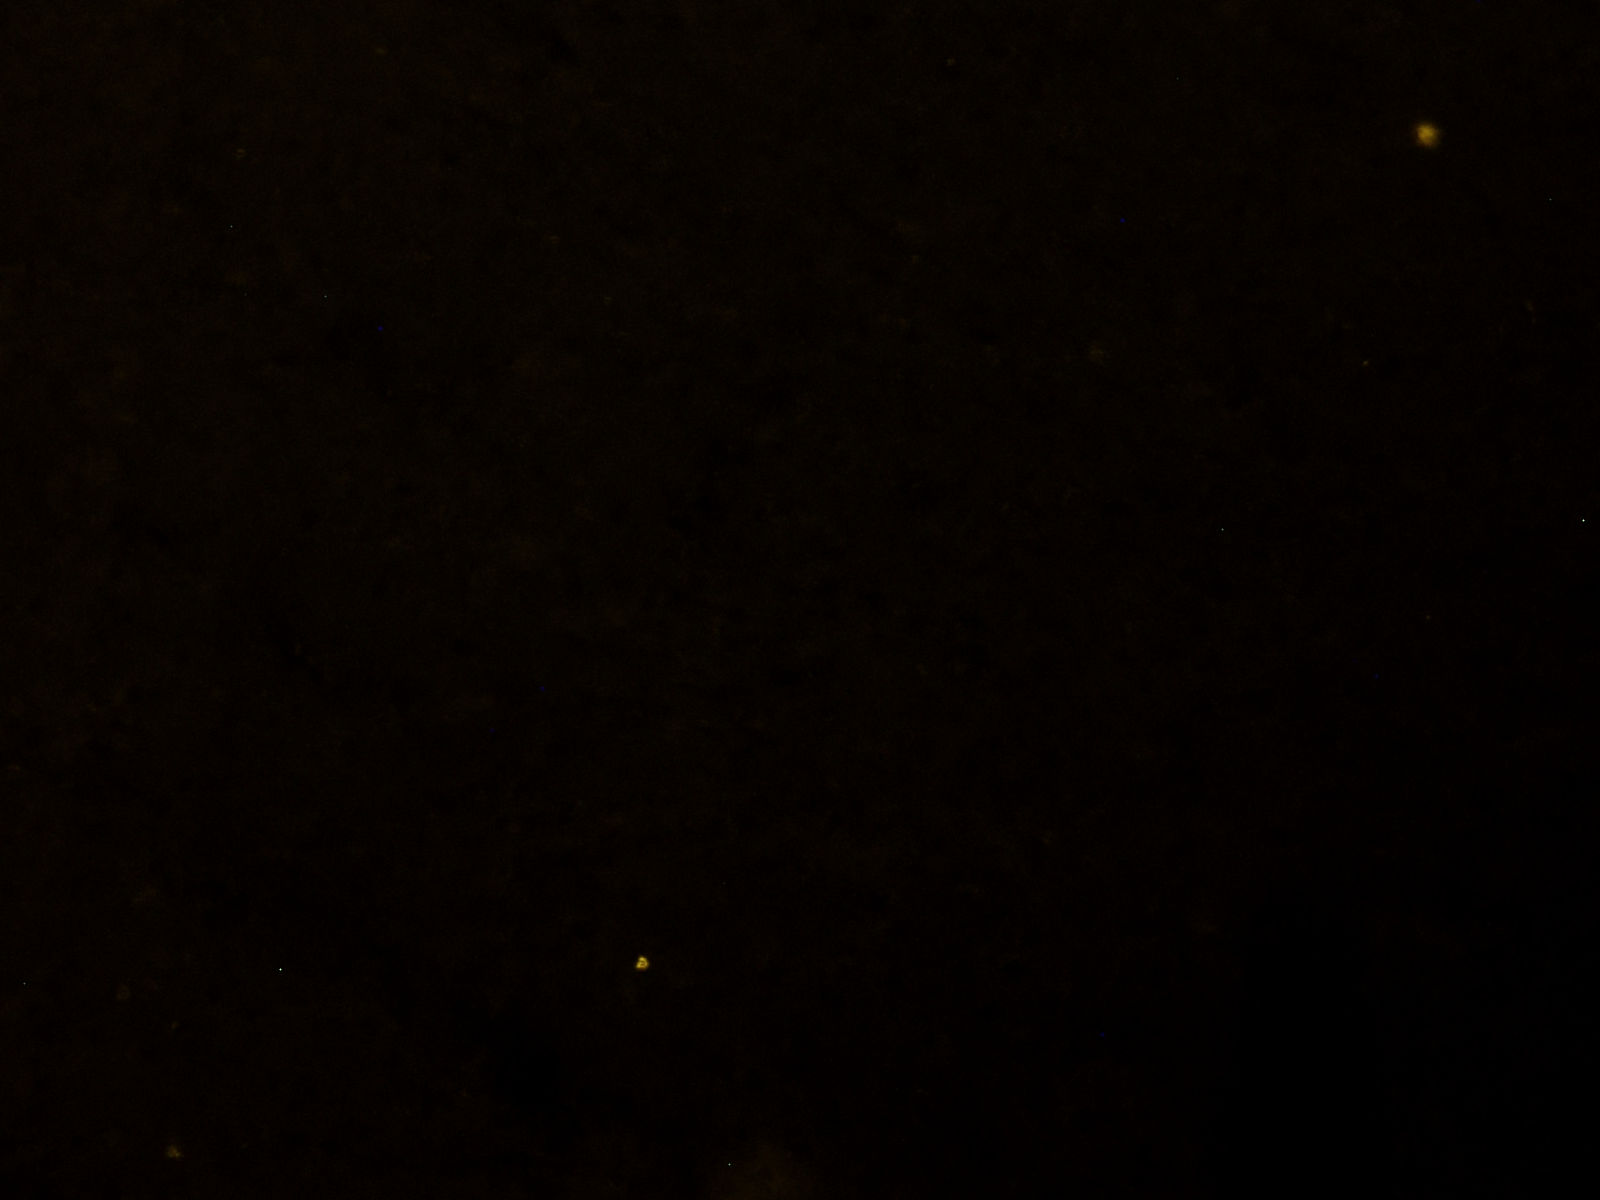
\includegraphics[width=0.5\linewidth]{figures/120_dataset/i_empty.png}

\includegraphics[width=0.5\linewidth]{figures/120_dataset/m_empty.png}
\subcaption{}
\label{fig:dataset:empty}
\end{subfigure}

\centering
\begin{subfigure}{1.1\textwidth}
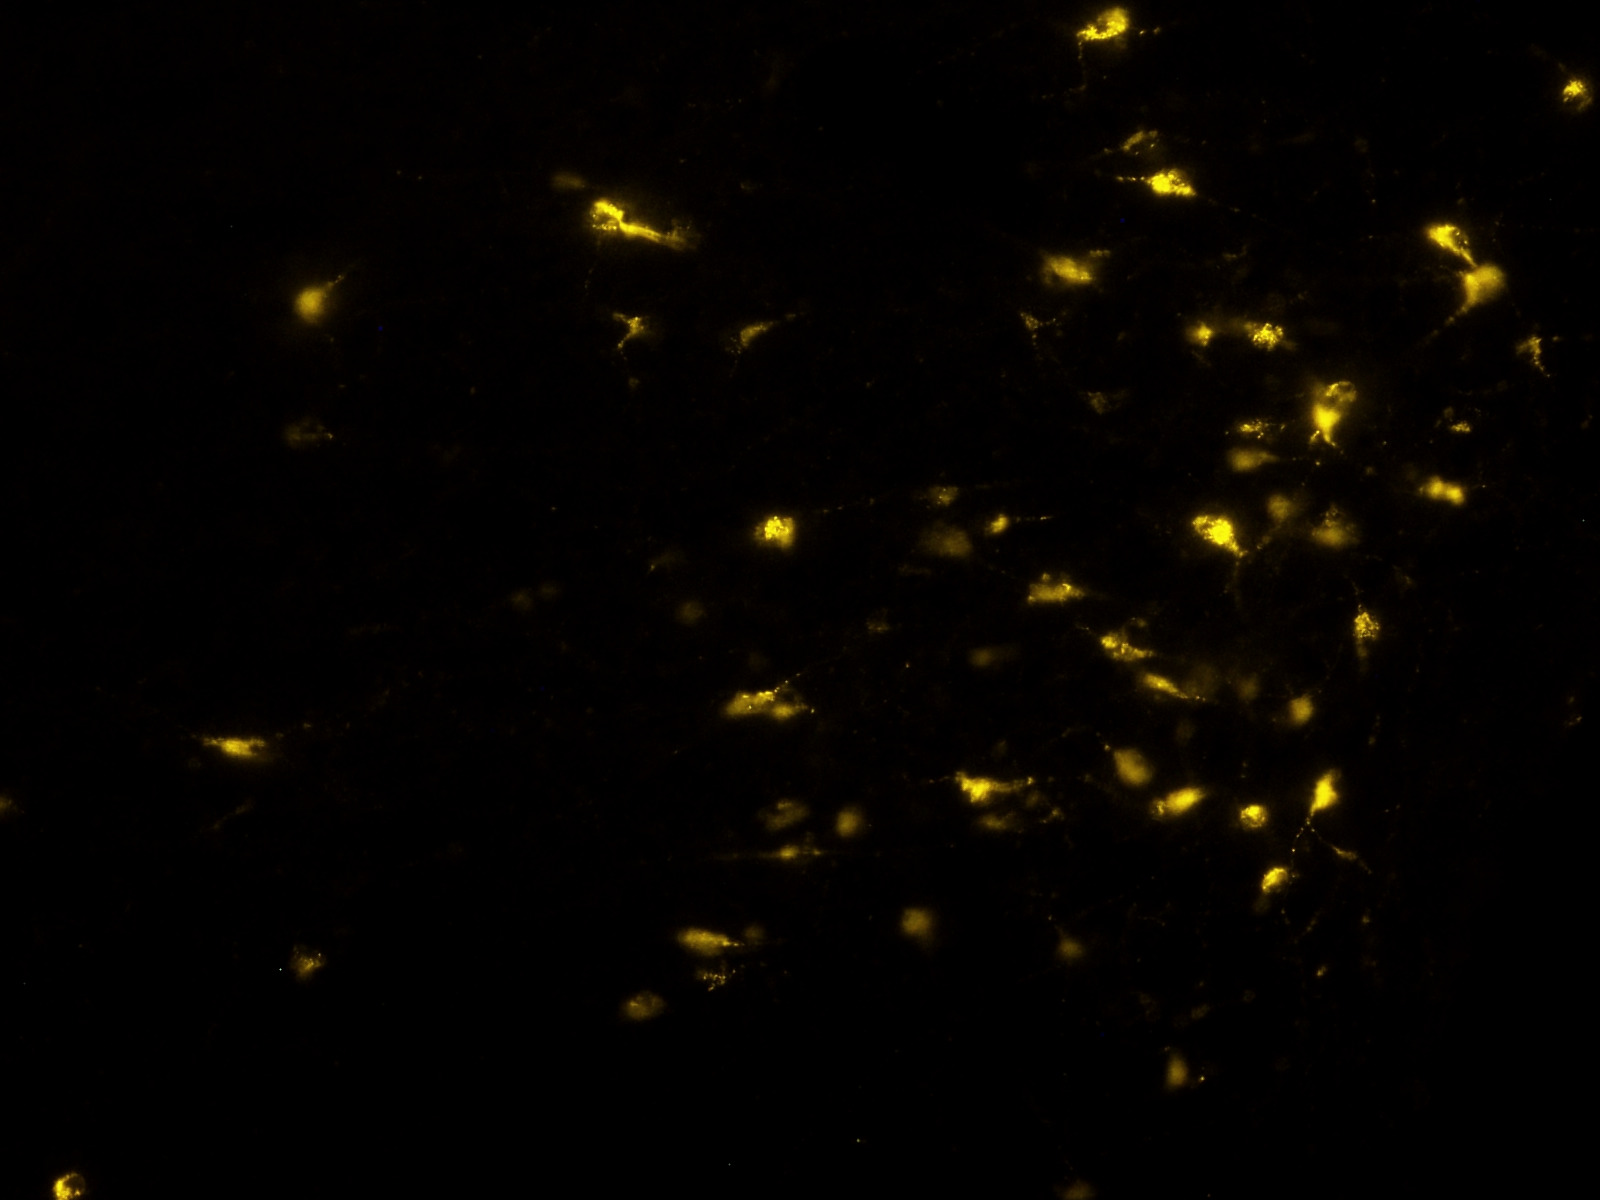
\includegraphics[width=0.5\linewidth]{figures/120_dataset/i_168.jpeg}
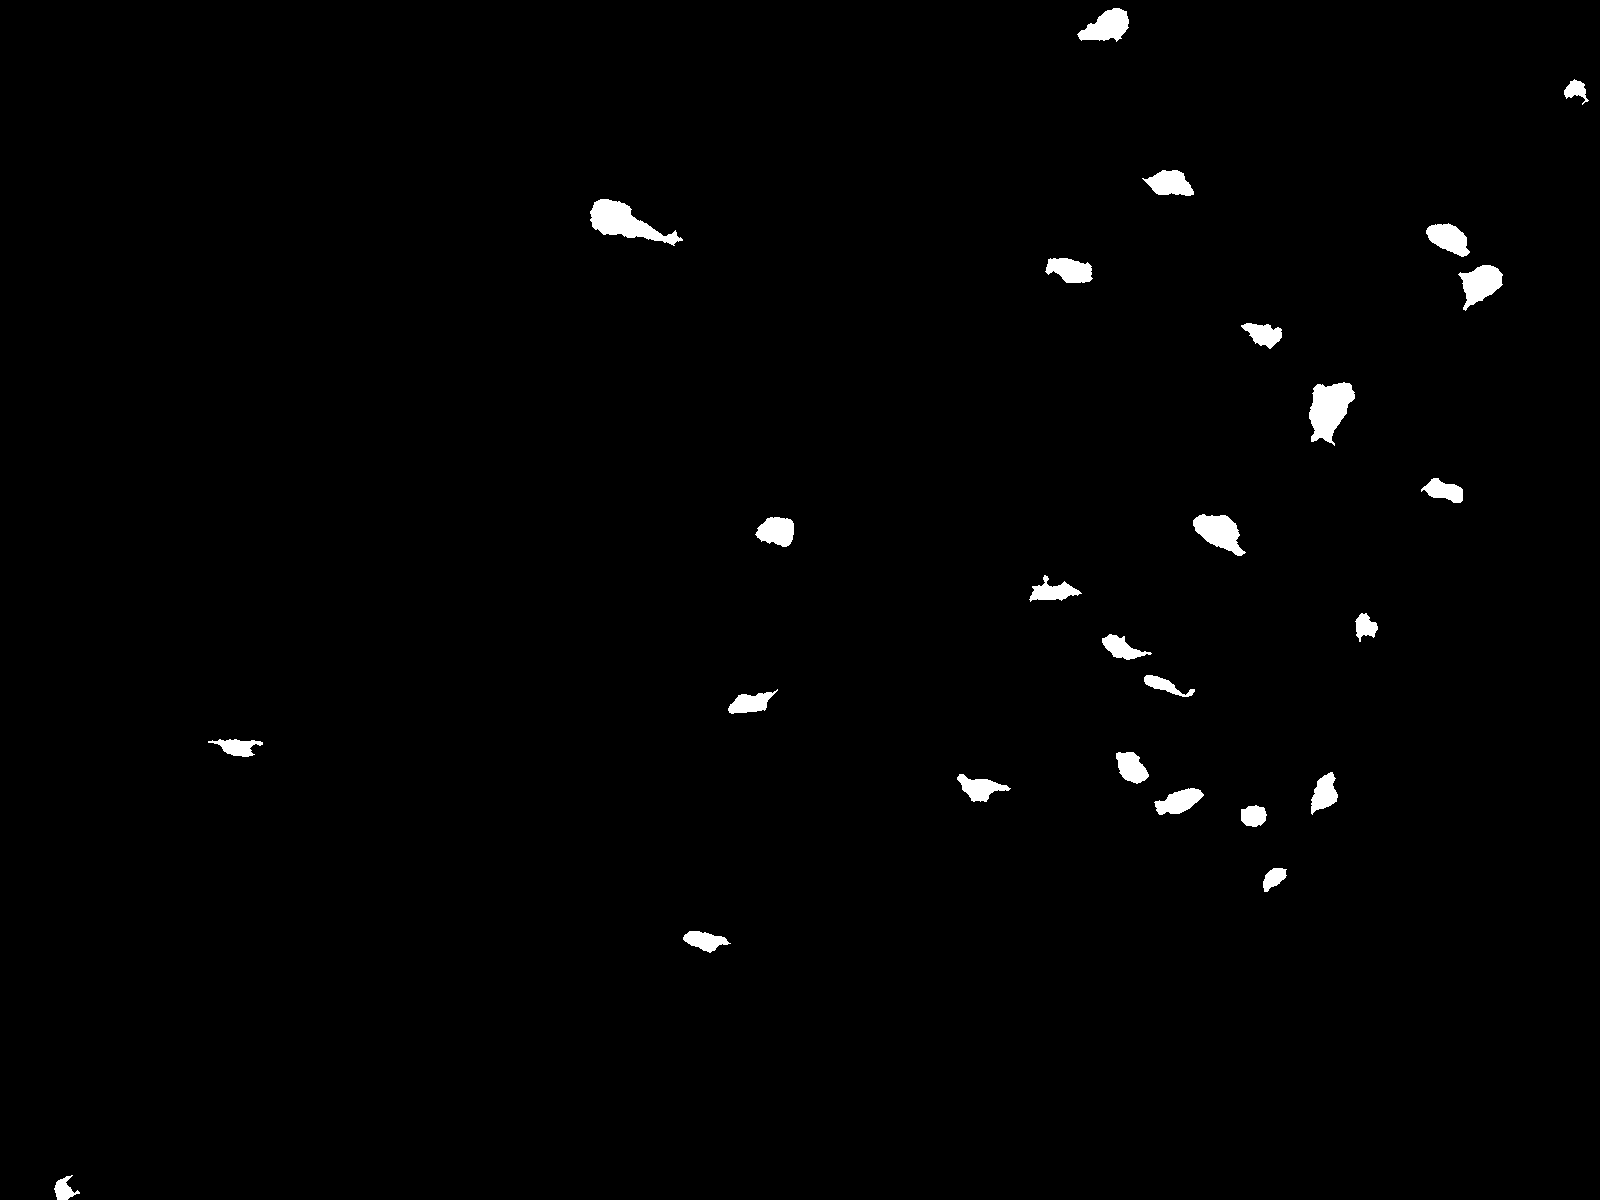
\includegraphics[width=0.5\linewidth]{figures/120_dataset/m_168.png}
\subcaption{}
\label{fig:dataset:dark}
\end{subfigure}

\centering
\begin{subfigure}{1.1\textwidth}
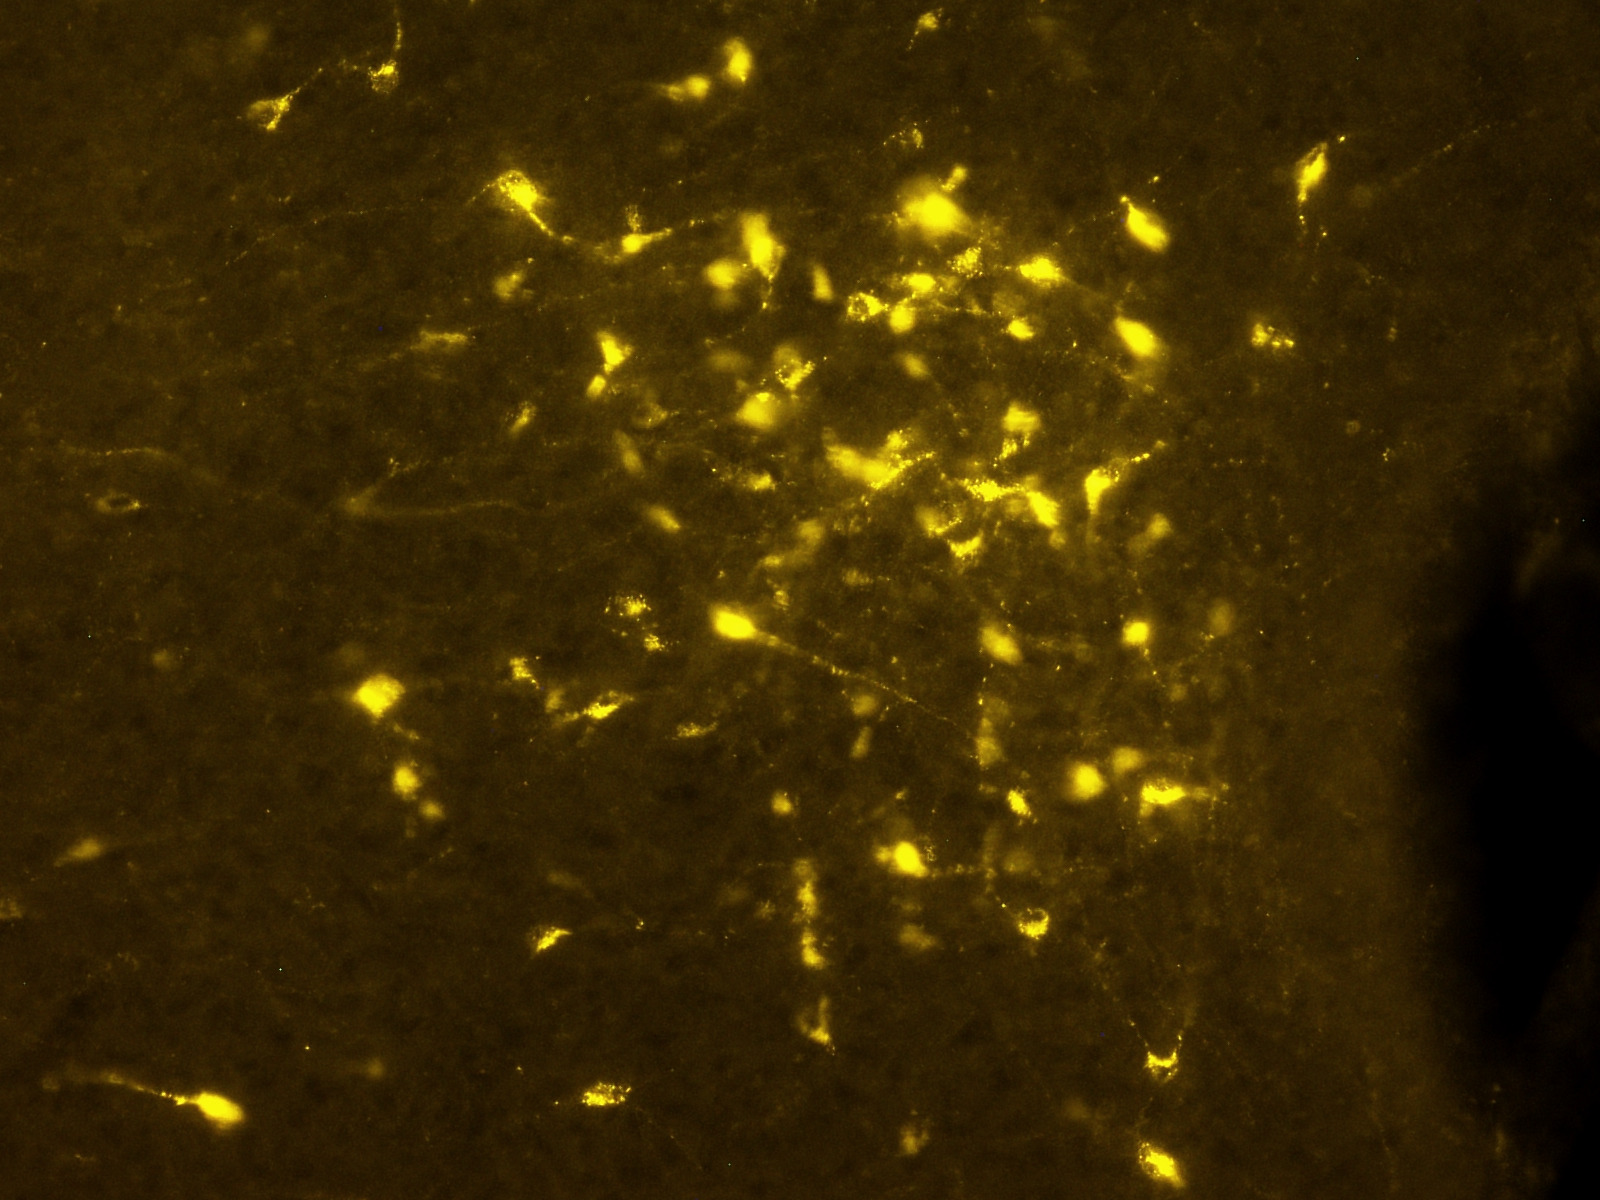
\includegraphics[width=0.5\linewidth]{figures/120_dataset/i_257.jpeg}
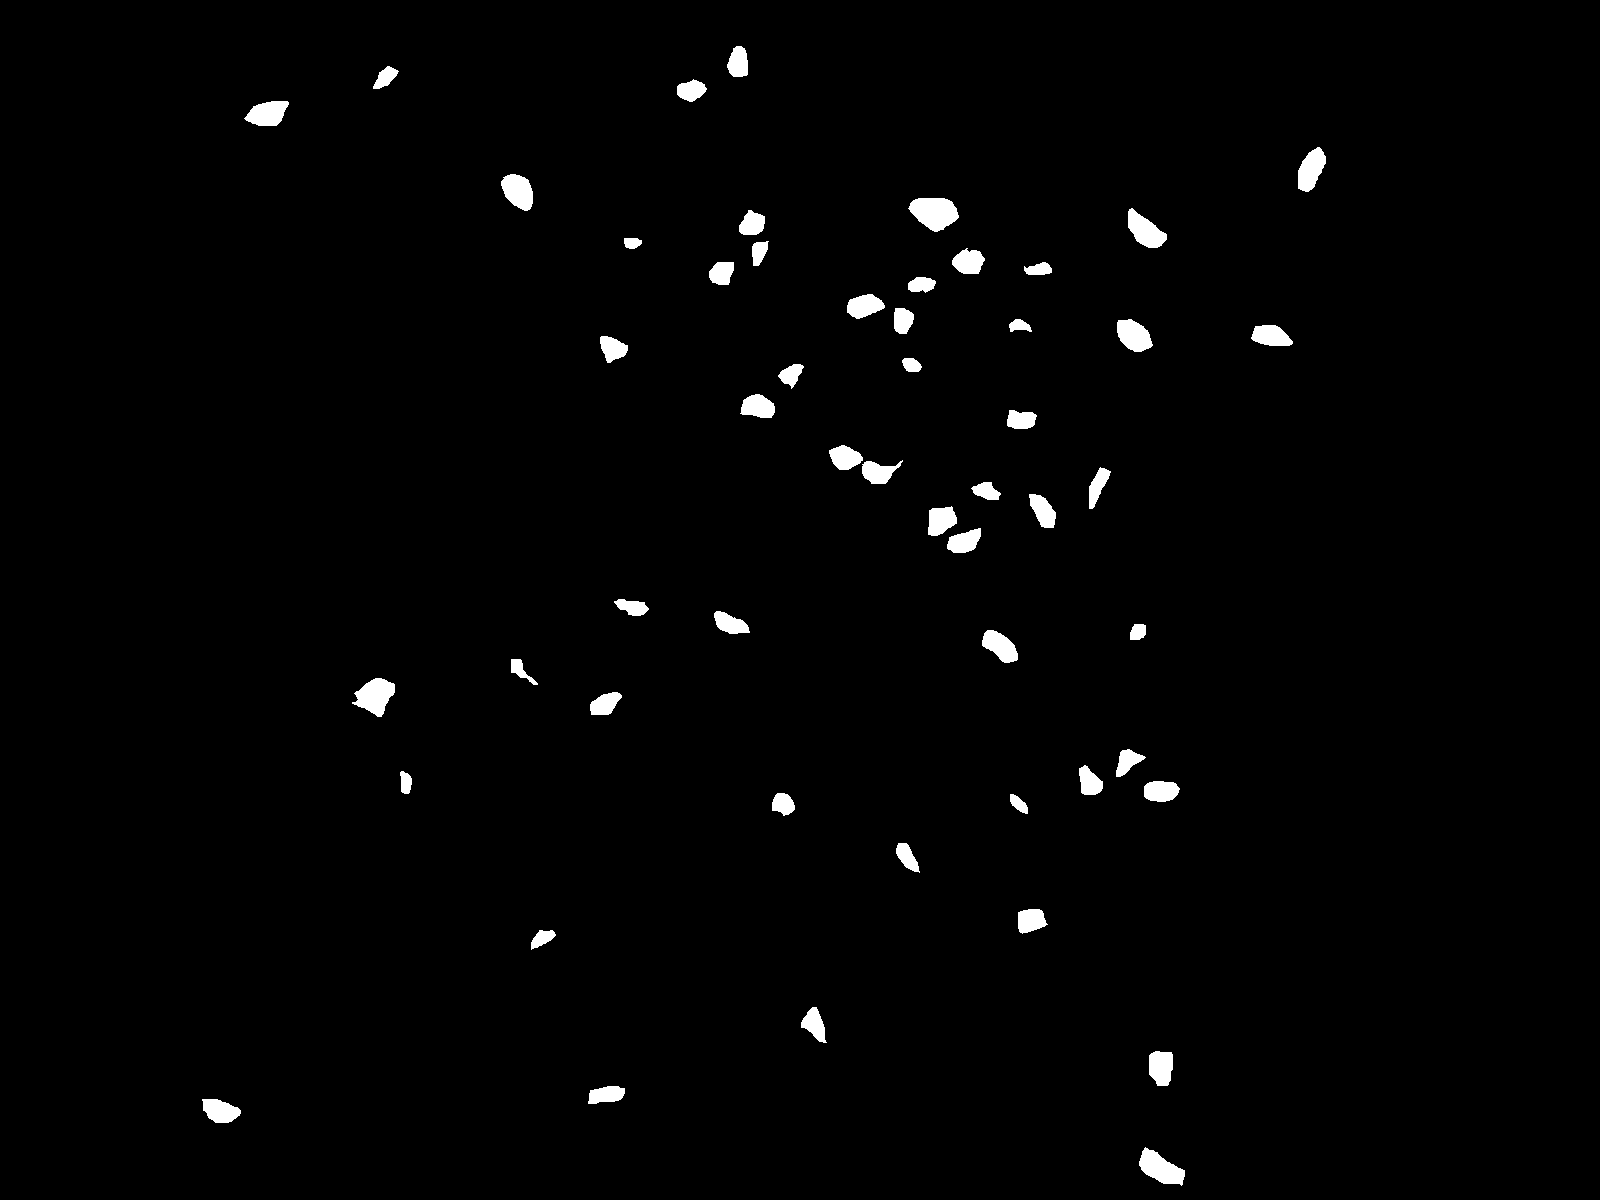
\includegraphics[width=0.5\linewidth]{figures/120_dataset/m_257.png}
\subcaption{}
\label{fig:dataset:bright}
\end{subfigure}
\vspace{-0.2cm}
\caption{
\textbf{Sample data}. 
Original images (left) and corresponding ground-truth masks used for training (right).
% The original images (left) present neuronal cells of different shape, size and saturation over a background of variable brightness and color.
% The corresponding ground-truth masks used for training (right) depicts cells as white pixels over a black background.
} \label{fig:dataset}
\end{figure}%
\begin{figure}%[ht]\ContinuedFloat
\centering
\begin{subfigure}{1.1\textwidth}
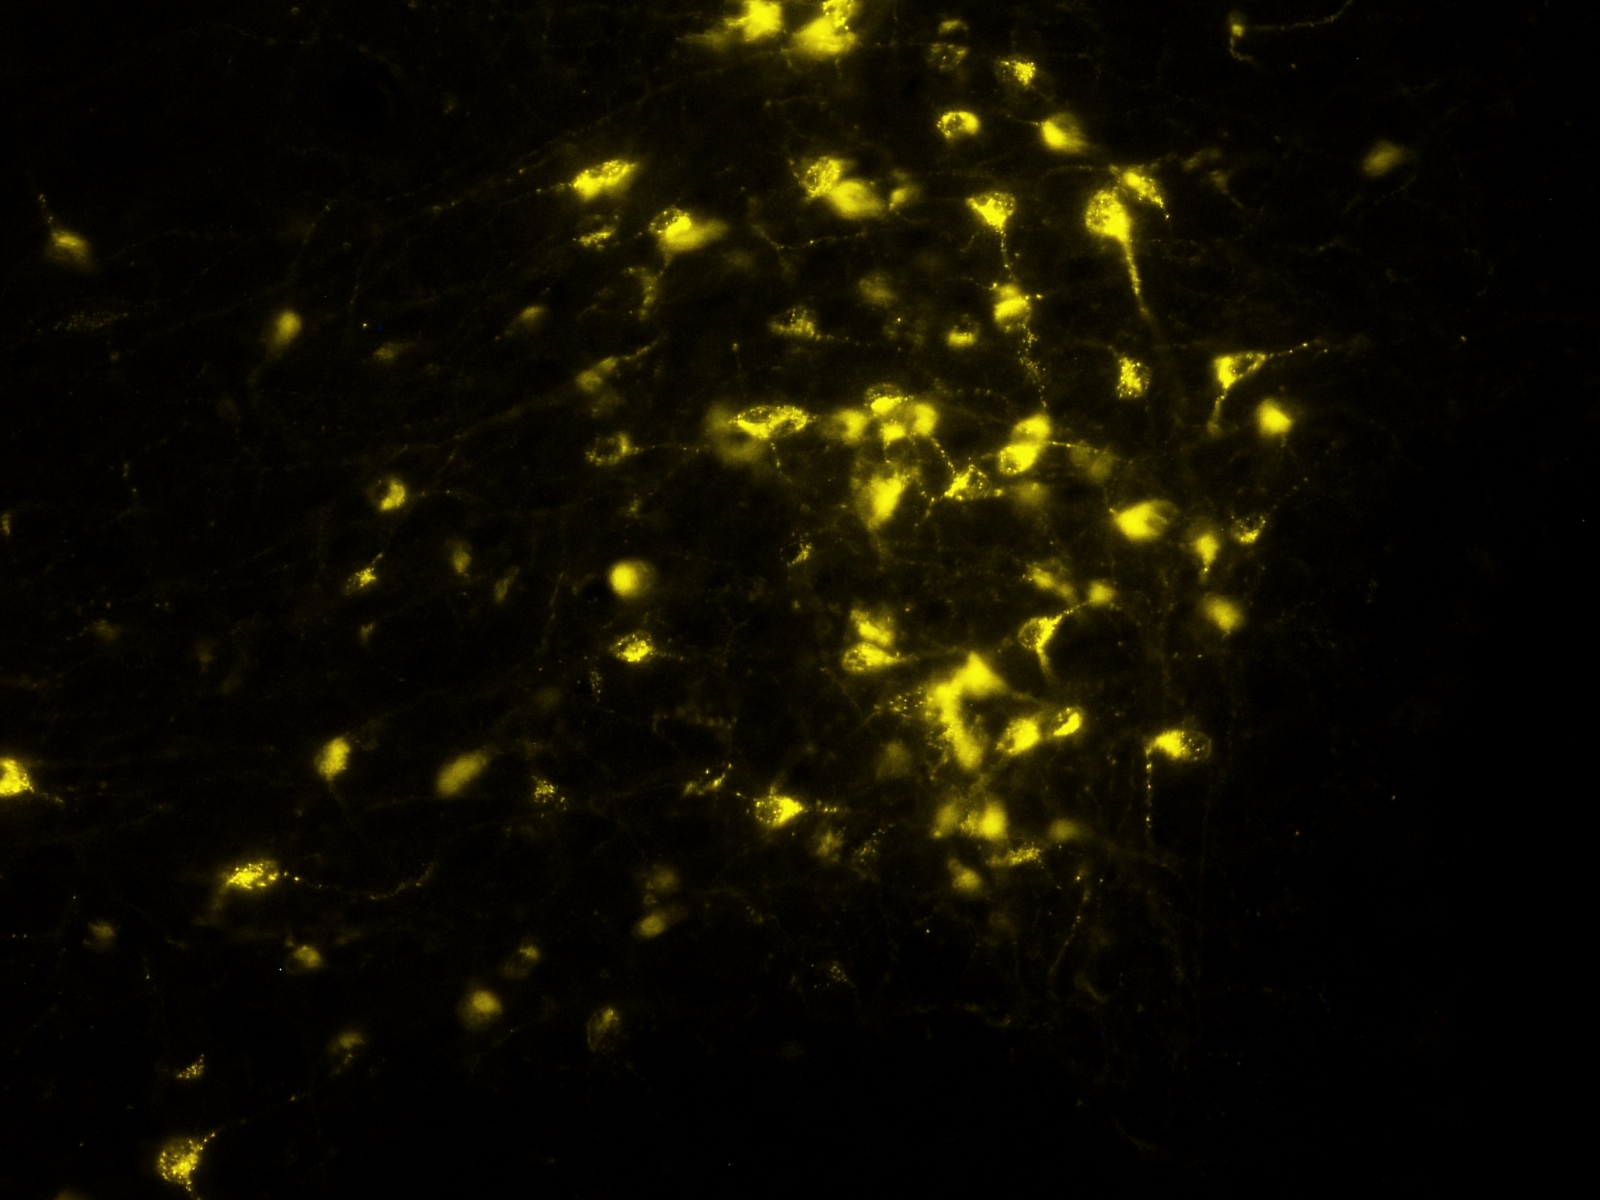
\includegraphics[width=0.5\linewidth]{figures/120_dataset/i_clumping_yellow.png}
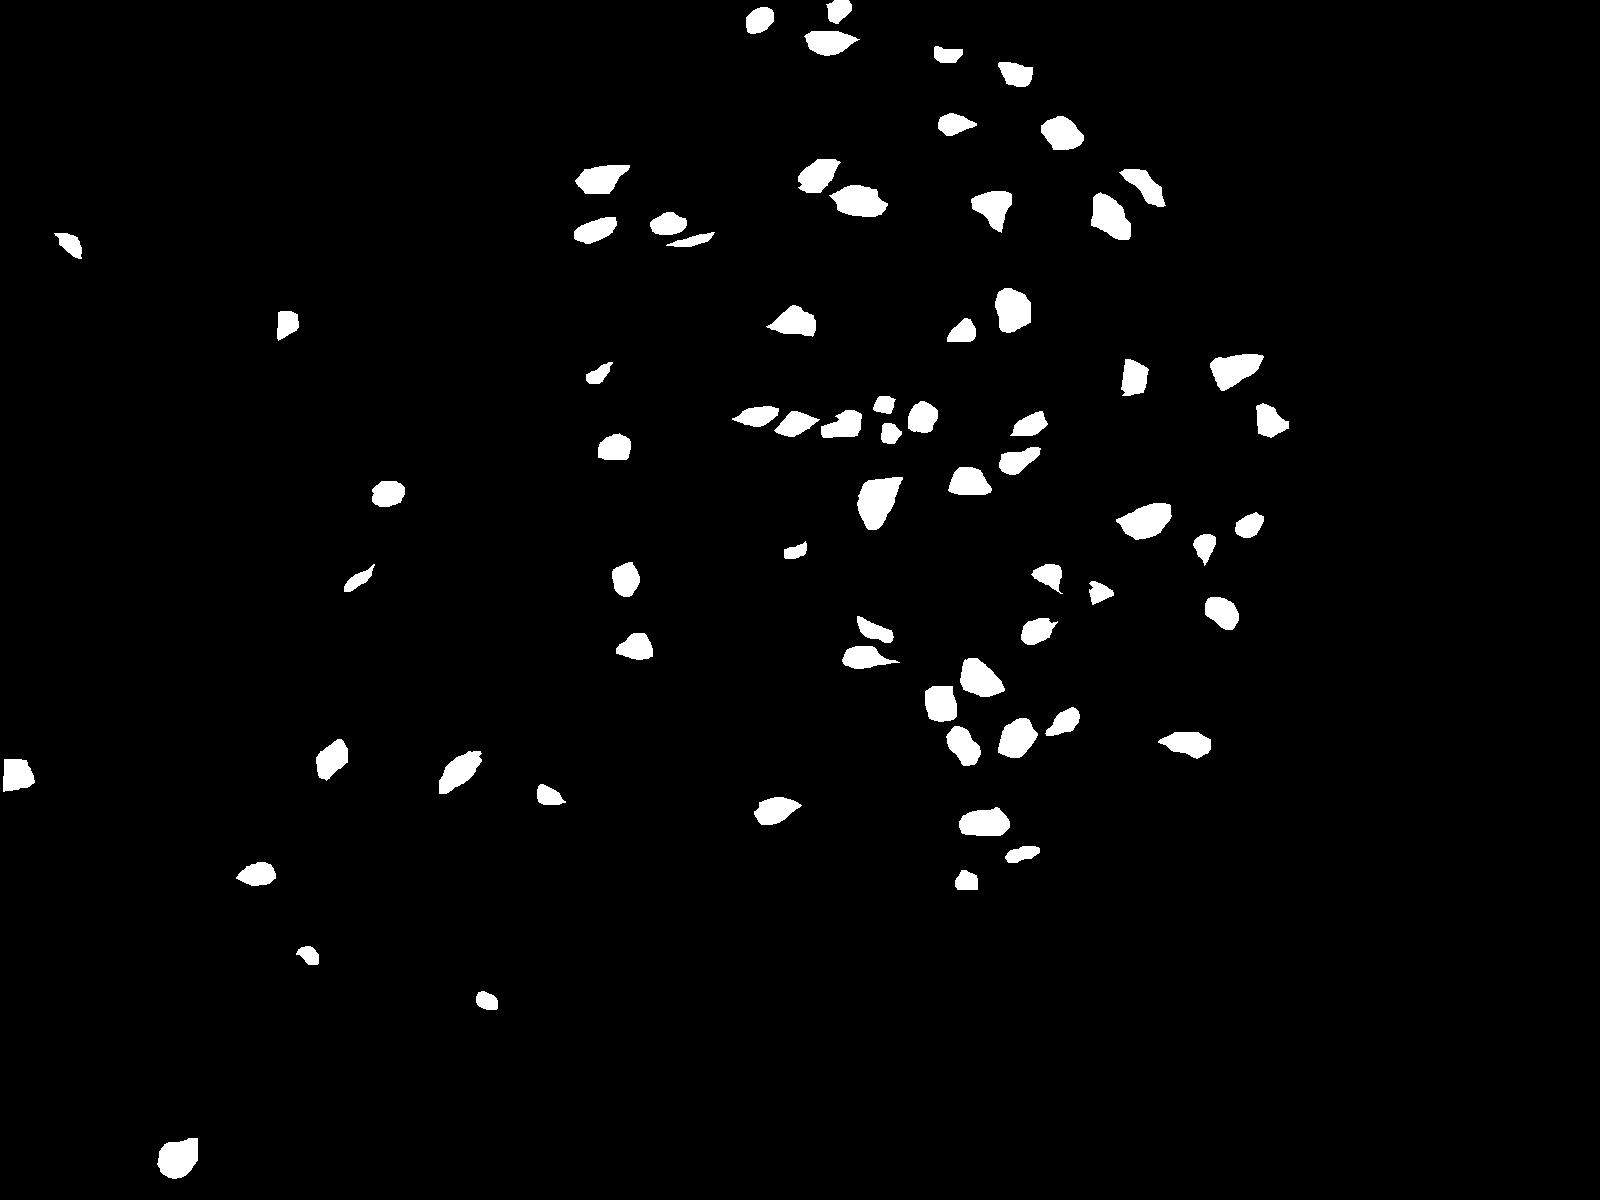
\includegraphics[width=0.5\linewidth]{figures/120_dataset/m_clumping_yellow.png}
\subcaption{}
\label{fig:artifacts:clumping}
\end{subfigure}

\centering
\begin{subfigure}{1.1\textwidth}
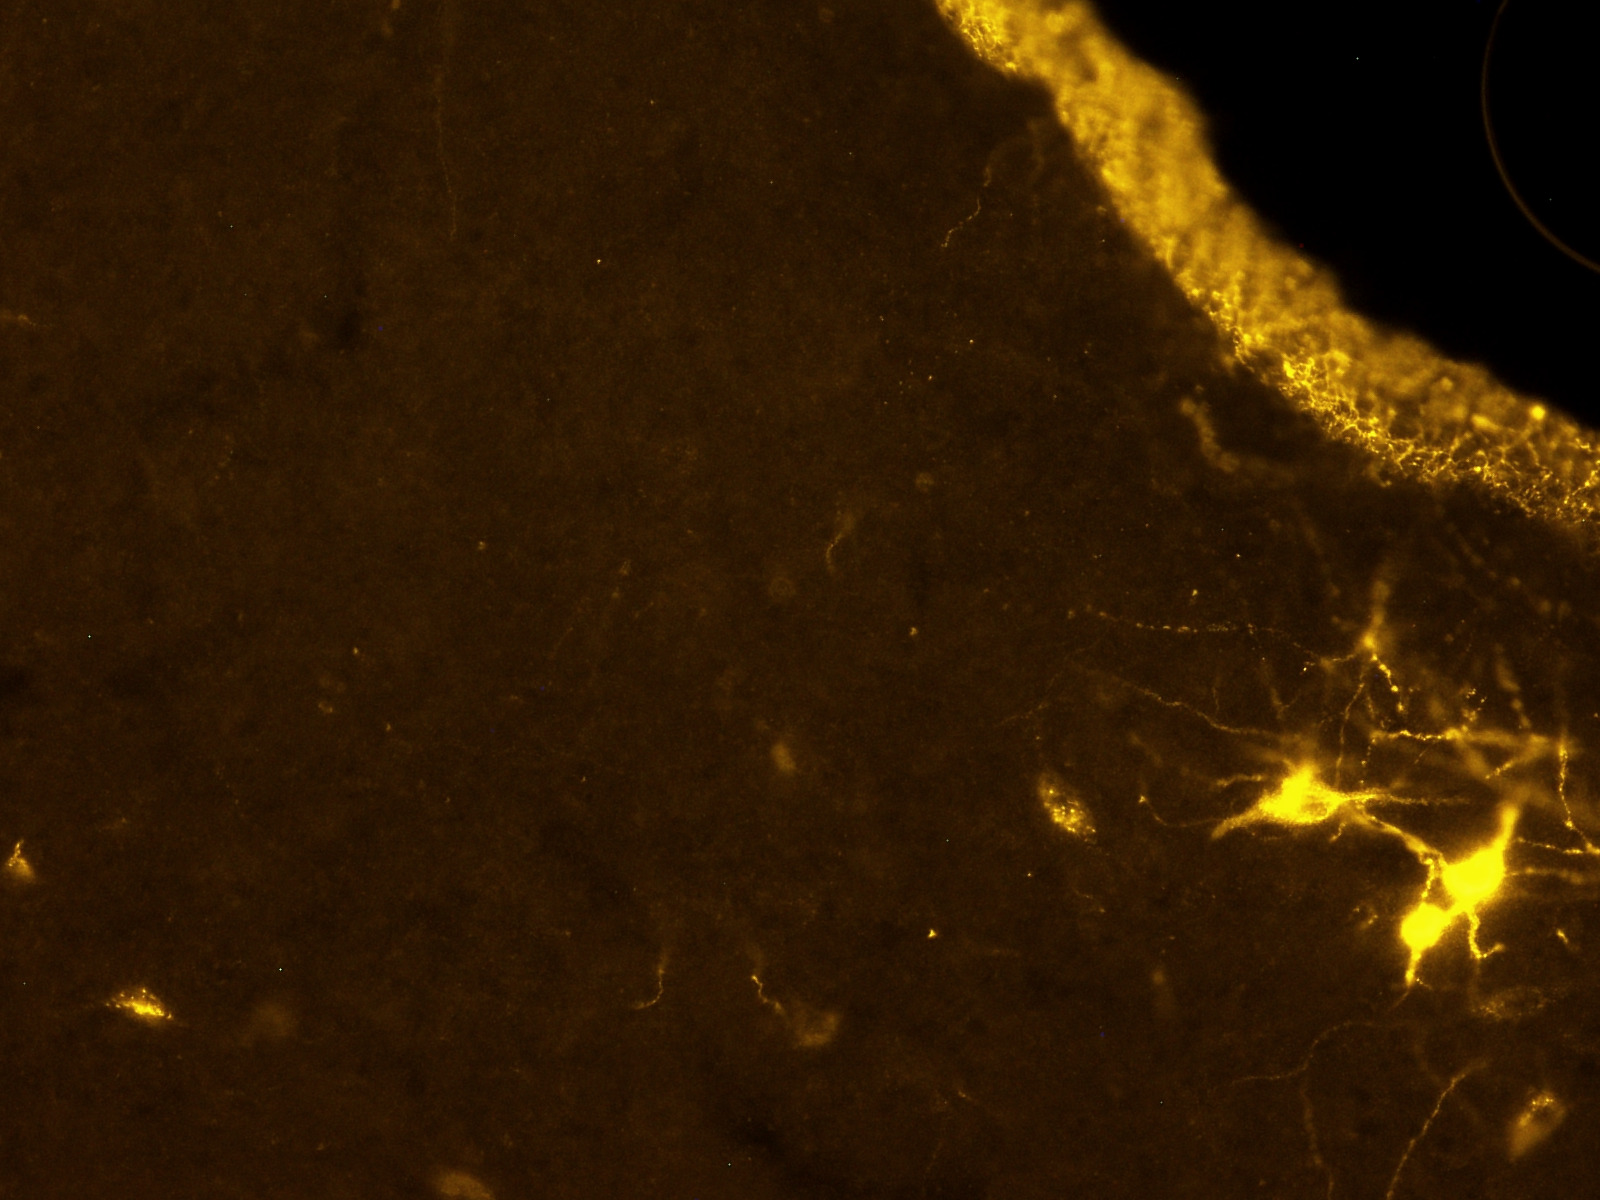
\includegraphics[width=0.5\linewidth]{figures/120_dataset/i_252.jpeg}
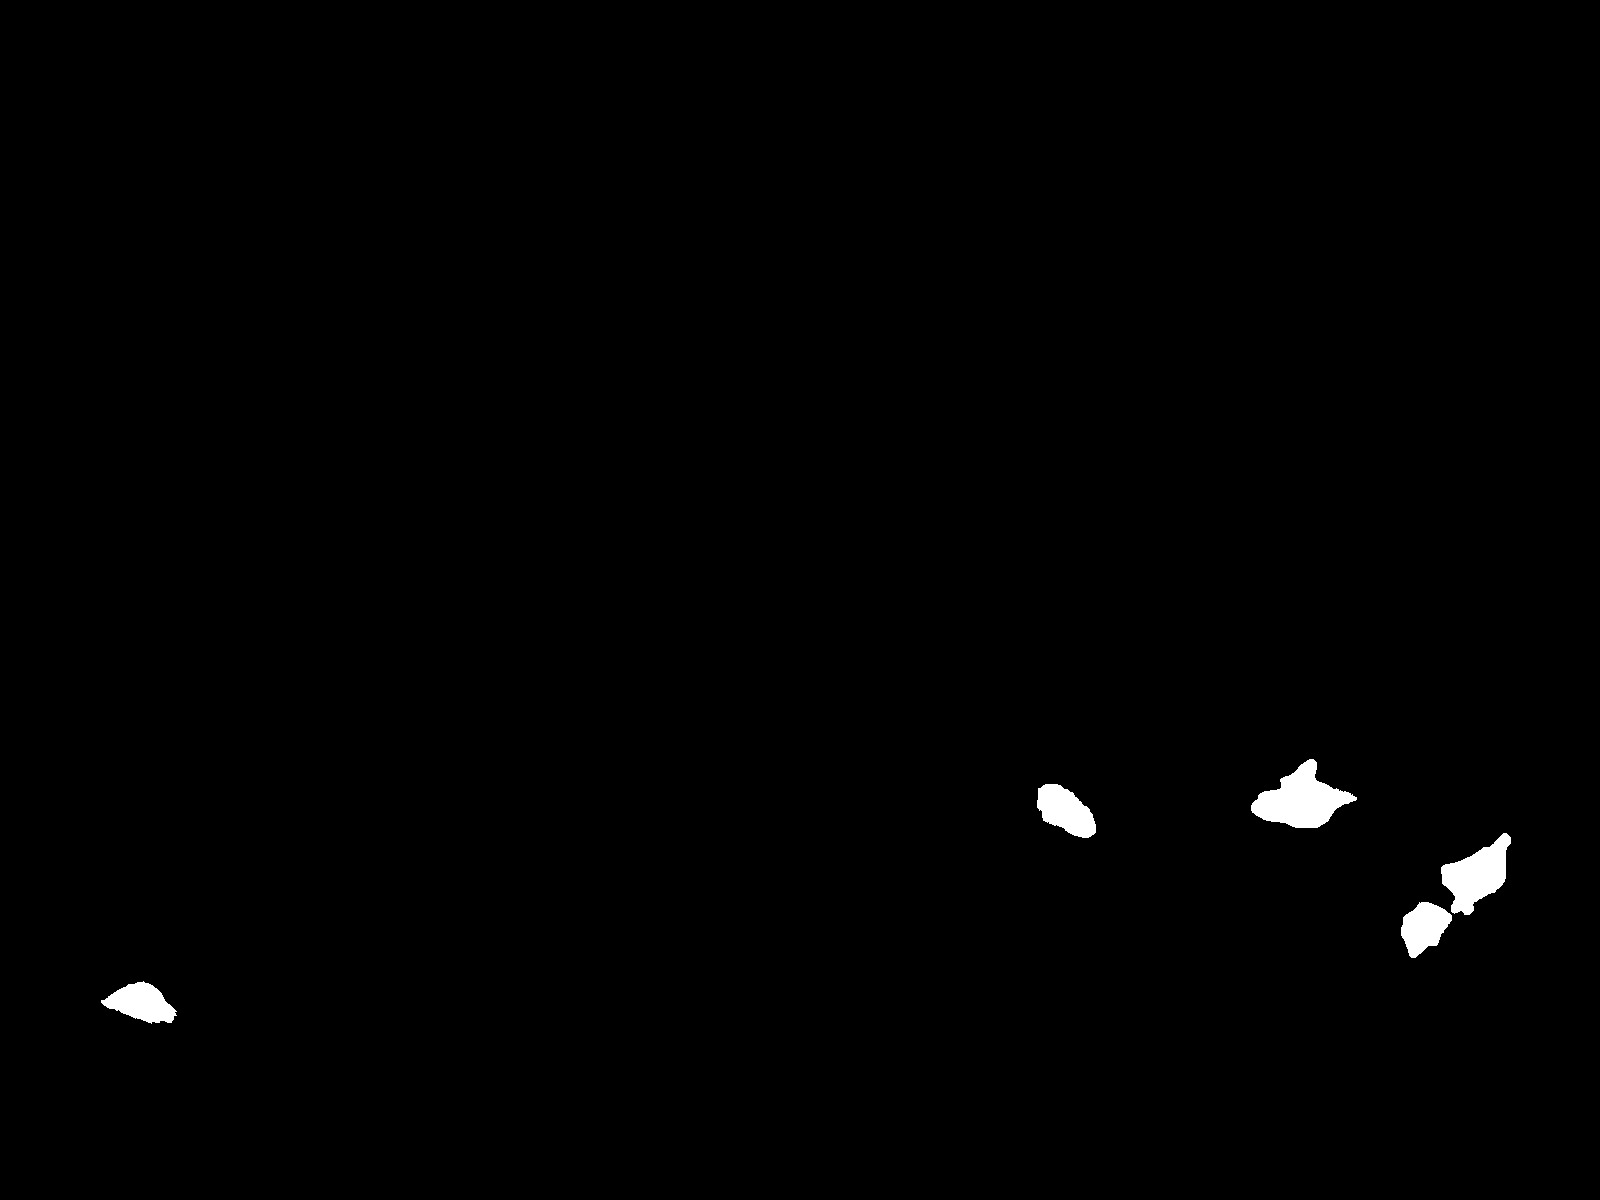
\includegraphics[width=0.5\linewidth]{figures/120_dataset/m_252.jpeg}
\subcaption{}
\label{fig:artifacts:stripe}
\end{subfigure}
\centering
\begin{subfigure}{1.1\textwidth}
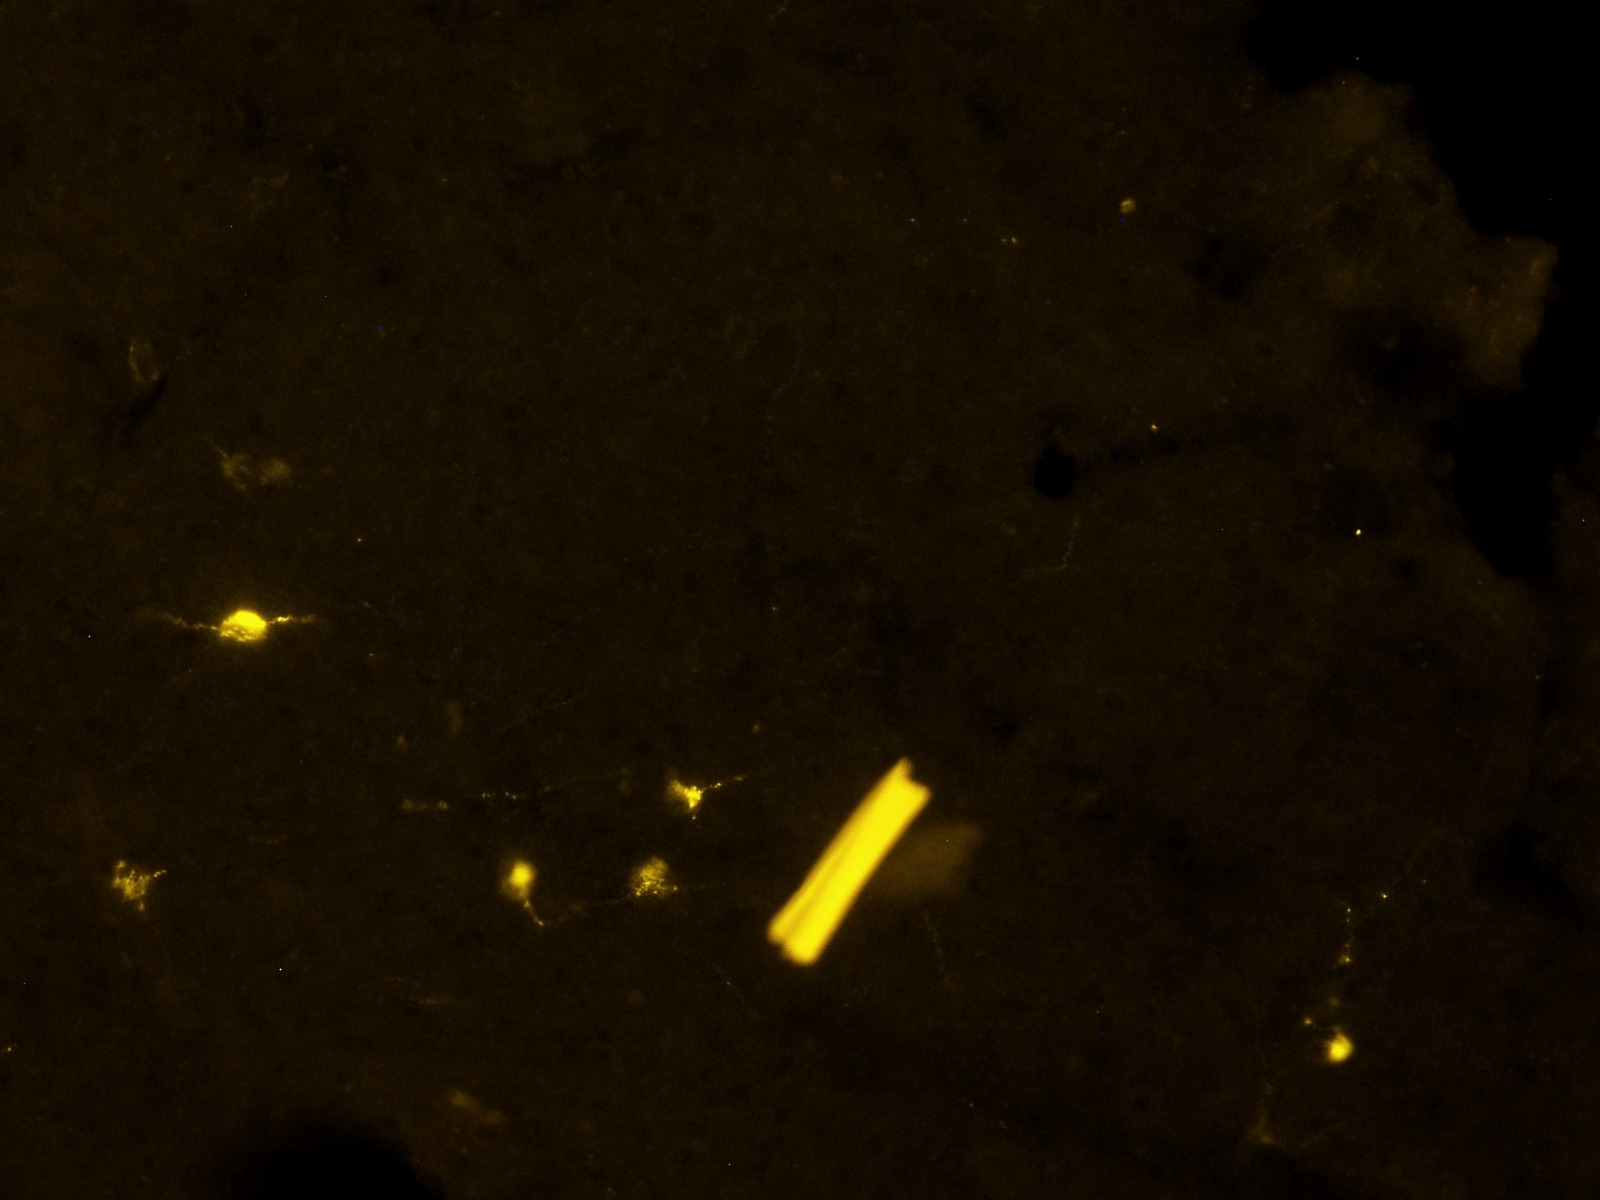
\includegraphics[width=0.5\linewidth]{figures/120_dataset/i_maccherone.jpeg}
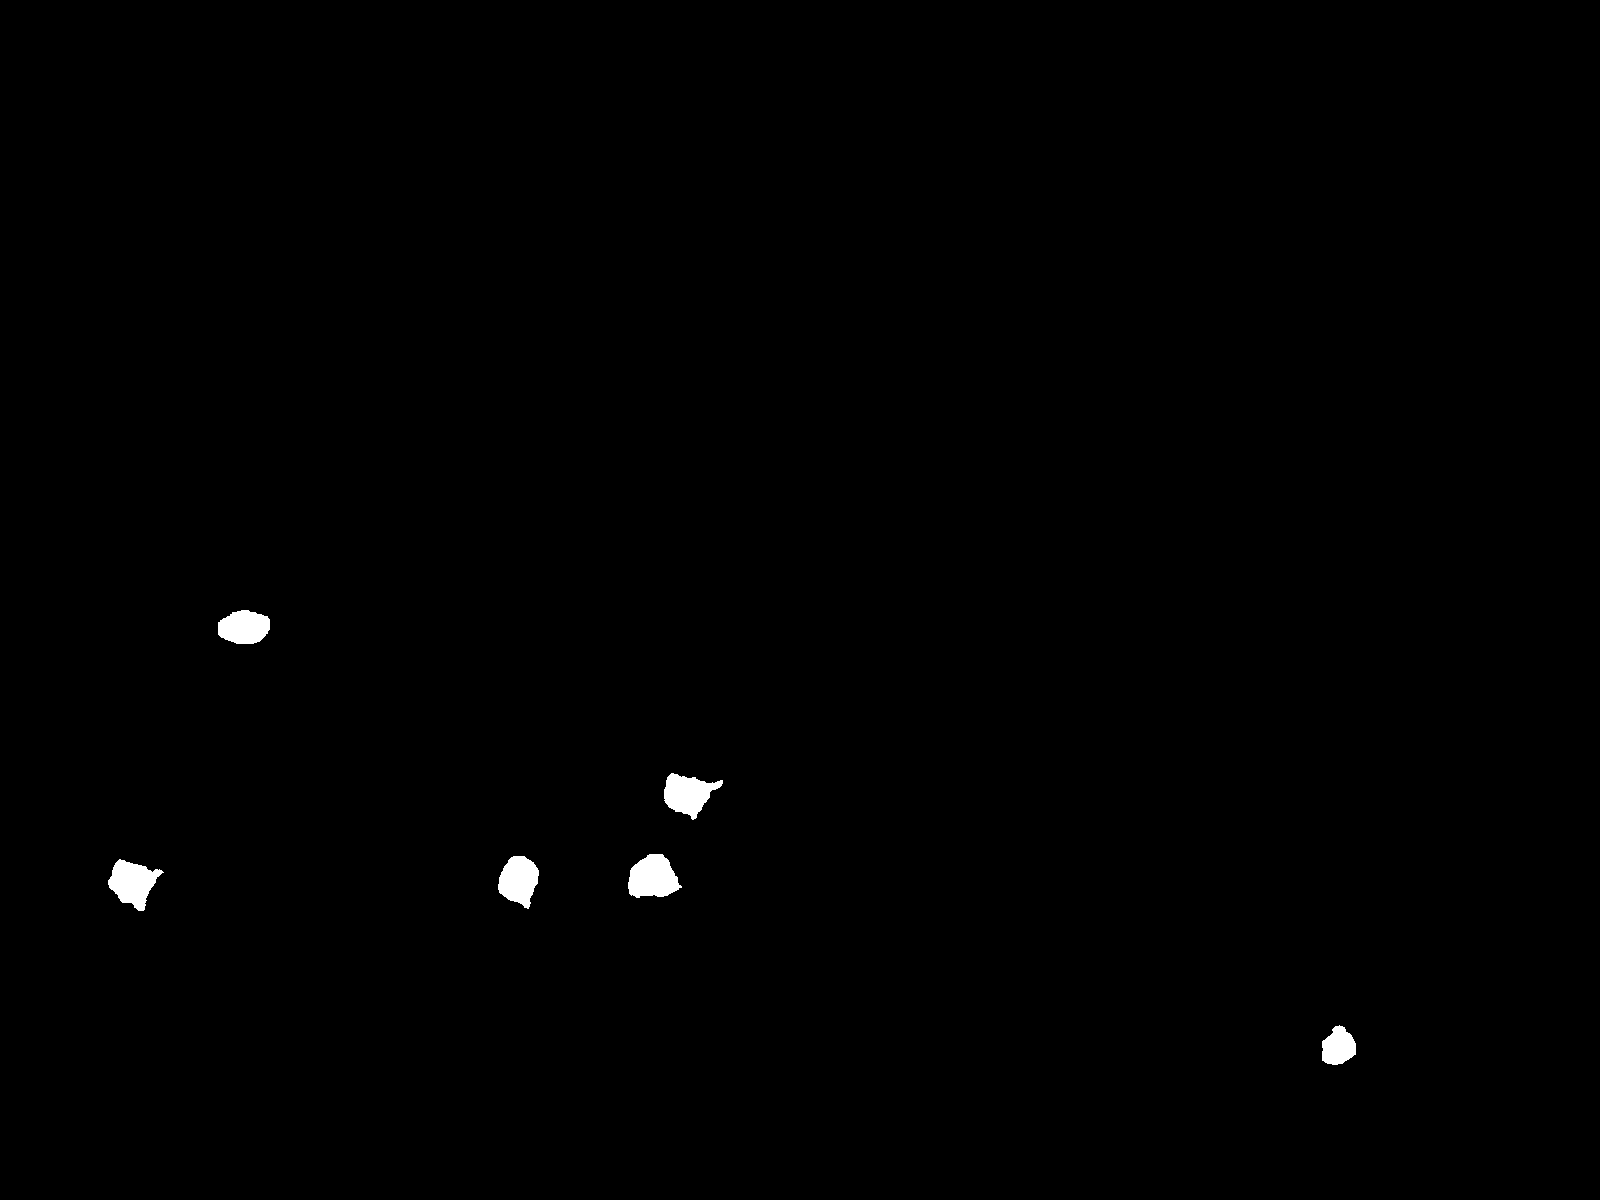
\includegraphics[width=0.5\linewidth]{figures/120_dataset/m_maccherone.png}
\subcaption{}
\label{fig:artifacts:macaroon}
\end{subfigure}
\vspace{-0.2cm}
\caption{
\textbf{Artifacts and challenges}. Neuronal cells appears of different shape, size and saturation over a background of variable brightness and color.
%%rephrase
% \textbf{Sample data}. In the original images (left), the neuronal cells of interest appear as yellow spots over a background of variable brightness and color. They exhibit a large variability in terms of shape, size and saturation, which makes them hard to distinguish from artifacts and similar biological structures that are not of interest.
% The corresponding ground-truth masks used for training (right) depicts cells as white pixels over a black background.
} 
\label{fig:artifacts}
\end{figure}

The \textbf{Fluorescent Neuronal Cells} dataset \cite{clissa2021fluocells} consists of 283 
% high-resolution 
pictures 
% (1600$\times$1200 pixels) 
of mice brain slices and the corresponding ground-truth labels.
In order to acquire these images, the mice were subjected to controlled experimental conditions, and a monosynaptic retrograde tracer (Cholera Toxin b, CTb) was surgically injected into brain tissues to highlight the neurons connected to the injection site
%projecting to the injection site
\cite{hitrec2019neural}.
Specimens of brain slices were then observed through  
a fluorescence microscope configured to select the narrow wavelength of light emitted by 
a fluorophore (of a yellow/orange color) associated with the tracer.
Thus, the resultant images depict neurons of interest as
% objects of different size and shape appearing as 
yellow-ish spots
% of variable brightness and saturation 
over a composite, generally darker background (\cref{fig:dataset,fig:artifacts}, left).

% Although many efforts were made to stabilize the acquisition procedure, the images present several relevant challenges for the detection task. 
% For example, the variability in brightness and contrast causes some fickleness in the pictures overall appearance (cfr. \cref{fig:dataset:dark,fig:dataset:bright}).  
% Also, the cells themselves exhibit varying saturation levels due to the natural fluctuation of the fluorescent emission properties (cfr. \cref{fig:dataset:dark,fig:artifacts:clumping}).
% Moreover, the substructures of interest have a fluid nature. This implies that the size and shape of the stained cells may change significantly (see \cref{fig:artifacts:clumping}, right), making it even harder to discriminate between them and the background. 
% Combined to that, artifacts (\cref{fig:artifacts:stripe,fig:artifacts:macaroon}), bright biological structures -- like neurons' filaments -- (\cref{fig:artifacts:stripe}) and non-marked cells similar to the stained ones handicap the recognition task. 
% Last but not least, another source of complexity is the broad shift in the number of target cells from image to image.
% Indeed, the total counts range from no stained cells (\cref{fig:dataset:empty}) to several dozens clumping together (\cref{fig:artifacts:clumping}). 
% As a consequence, this requires a model with both high precision -- to prevent false positives in the former case -- and high recall -- since considering two or more touching neurons only once produces false negatives.
% % In the former case, the model needs high precision in order to prevent false positives. The latter, instead,
% % requires high recall since considering two or more touching neurons only once produces false negatives. 

% By and large, all of these factors make the recognition and counting tasks more problematic and complicate the model training.
% Likewise, these challenges hinder model evaluation as the interpretation of such borderline cases becomes subjective.

\section{Data exploration}
\label{sec:data_exploration}

Fluorescent Neuronal Cells images are high-resolution RGB pictures of constant shape (1200 pixels height by 1600 pixels width) collected under fixed experimental conditions.
% In terms of data features, the most interesting aspects regard the color and luminance information, the counts distribution and the cells characteristics.
% In terms of data features, the most interesting aspects pertain the color and luminance information, the counts' distribution and characteristics of the cells.
The data can be explored at two complementary levels: pixel features and cell characteristics. 
On the one hand, interesting insights can be retrieved by looking at pixels' color and luminance information. Also, analogous analyses on the ground-truth masks reveal essential information about class-imbalance between signal and background.
On the other hand, examining object properties can highlight potential nuisances and suggest how to evaluate model performances.

The above data explorations are presented in the following sections of this chapter, and a summary table of the most important data features is reported in \cref{tab:data_features}.
\renewcommand{\cellalign}{cc}
\renewcommand{\theadalign}{cc}
\begin{table}[]
    \centering
    \resizebox{\textwidth}{!}{
    % \begin{tabular}{lrrrrrrrr}
    % \toprule
    % {} &          \thead{red\\intensity} &        \thead{green\\intensity} &         \thead{blue\\intensity} &  signal (\%) &  signal ratio &     area &  \thead{Feret\\diameter} &  \# cells \\
    % \midrule
    % mean &   7.32 &   2.83 &  0.20 &        0.50 &    366,681.94 & 1,212.18 &           55.71 &    27.05 \\
    % \thead{standard\\deviation}  &  16.81 &  13.30 &  1.43 &        0.61 &    755,628.42 &   995.40 &           26.12 &    21.75 \\
    % min  &   0 &   0 &  0 &        0 &         19.57 &   162 &           18.68 &     0 \\
    % 10\%  &   0 &   0 &  0 &        0 &         92.39 &   358 &           30.02 &     4 \\
    % 25\%  &   2 &   0 &  0 &        0.09 &        145.35 &   564 &           38.08 &     7 \\
    % 50\%  &   5 &   1 &  0 &        0.34 &        291.10 &   913 &           49.50 &    21 \\
    % 75\%  &   9 &   2 &  0 &        0.68 &      1,163.29 & 1,504 &           66.48 &    48 \\
    % 90\%  &  12 &   4 &  0 &        1.07 &  1,920,000 & 2,409 &           88.02 &    59 \\
    % max  & 252 & 251 & 87 &        4.86 &  1,920,000 & 8,092 &          215.10 &    68 \\
    % \bottomrule
    % \end{tabular}
    
    \begin{tabular}{lrrrrrrrr}
    \toprule
    {} &          \thead{red\\intensity} &        \thead{green\\intensity} &         \thead{blue\\intensity} &  signal (\%) &  signal ratio &     area &  \thead{Feret\\diameter} &  \# cells \\
    \midrule
    count & 1,919,905 & 1,919,910 & 1,919,955 &      283 &        283 & 2,137 &        2,137 & 2,193 \\
    mean  &         7.32 &         2.83 &         0.20 &        0.50 &    366,681.94 & 1,212.18 &           55.71 &    27.05 \\
    \thead{standard\\deviation}   &        16.81 &        13.30 &         1.43 &        0.61 &    755,628.42 &   995.40 &           26.12 &    21.75 \\
    min   &         0 &         0 &         0 &        0 &         19.57 &   162 &           18.68 &     0 \\
    10\%   &         0 &         0 &         0 &        0 &         92.39 &   358 &           30.02 &     4 \\
    25\%   &         2 &         0 &         0 &        0.09 &        145.35 &   564 &           38.08 &     7 \\
    50\%   &         5 &         1 &         0 &        0.34 &        291.10 &   913 &           49.50 &    21 \\
    75\%   &         9 &         2 &         0 &        0.68 &      1,163.29 & 1,504 &           66.48 &    48 \\
    90\%   &        12 &         4 &         0 &        1.07 &  1,920,000 & 2,409 &           88.02 &    59 \\
    max   &       252 &       251 &        87 &        4.86 &  1,920,000 & 8,092 &          215.10 &    68 \\
    \bottomrule
    \end{tabular}
    }
    \caption{\textbf{Distributions summary.} 
    Summary of the distributions illustrated in \cref{sec:data_exploration}. For each distribution we report the mean and standard deviation; minimum, maximum and 10\textit{-th}, 25\textit{-th}, 50\textit{-th}, 75\textit{-th} and 90\textit{-th} percentiles; the count of objects from which such measures are computed, i.e. pixels, images and cells.
    Notice that \textit{\# cells} count is obtained from the 2137 cells plus the 56 empty images.
    % Notice that commas are used as thousands separator
    }
    \label{tab:data_features}
\end{table}

\subsection{Salient features}
\label{sec:data_features}

% As far as the color, t
The picture appearance is dominated by two prevalent tints due to the intentional selection of a specific wavelength: a darker hue corresponding to areas whose light was filtered out and a yellow tone emitted by the fluorophore
(\cref{fig:dataset:empty,fig:artifacts}).
As a consequence, the only color channels to be populated are red and green, while blue is typically empty. 
An example of this effect is reported in \cref{fig:dataset:pixel_intensity}, where the average distribution of pixel intensity is illustrated (log scale).
\begin{figure}
    \centering
    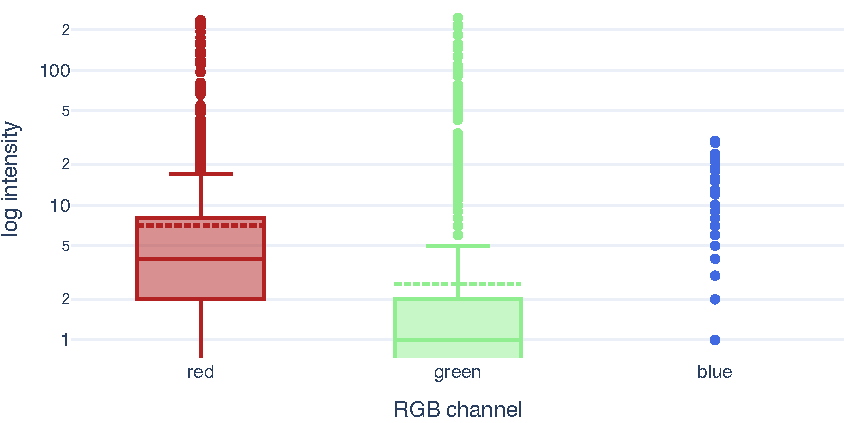
\includegraphics[width=\textwidth]{figures/120_dataset/features/pixel_intensity_distribution.pdf}
    \caption{\textbf{Pixel intensity distribution.} Violin plot of the average distribution of pixel intensities across the  RGB channels}
    \label{fig:dataset:pixel_intensity}
\end{figure}
In practice, the blues have an extremely narrow distribution squashed on zero, which makes it even difficult to visualize -- in fact only outliers are visible. 
The red and green channels are instead more populated. Their central tendency is still concentrated on low values due to the prevalence of background pixels, however we observe longer and thicker right tails, especially for the red channel (see \textit{red}, \textit{green} and \textit{blue} columns in \cref{tab:data_features} for a numeric summary).
Guided by this observation, one may argue that all this information is superfluous, so resorting to a grayscale transformation could be better since the images are ultimately shades of yellow.
A nice way to visually investigate such relationships is by exploring the colorspace representations of several images.
\Cref{fig:dataset:colorspace} reports the RGB and HSV encodings for two randomly sampled images.
Indeed, the RGB representations (\cref{fig:dataset:colorspace:rgb1,fig:dataset:colorspace:rgb2}) corroborate the previous intuition, as most pixels lay almost on a straight line in the red-green plane. 
This suggests that the two channels are highly correlated, so a one-dimensional subspace may be enough to represent most of the variability of the data.
In turn, this would bring two advantages: ease the learning process -- as neural networks typically suffer when inputs are correlated %\cite{} 
-- and make it more efficient -- as only one channel is considered instead of three.

However, the use-case at hand has no stringent requirements in terms of computing resources and runtime, so the 3-channels training is still feasible.
More importantly, the information thrown away when converting to grayscale, although tiny, may be crucial to discriminate background and signal. 
Hence, a 3D-encoding may still be worthed but the RGB colorspace may not be the optimal representation to learn this separation. A hint of that is demonstrated in \cref{fig:dataset:colorspace:hsv1,fig:dataset:colorspace:hsv2}, where the same images are depicted according to the HSV encoding. 
In this case, the separation between dark and colored tones appears more evident. 
Moreover, most of the pixels are concentrated in low hue values
and their distribution seems more spread across the saturation-value plane. 

All that being considered, we try to leverage the insights of both approaches. 
On one side, the RGB colorspace is taken as a starting point to retain all available information. On the other, the model first layer is designed to incorporate a colorspace transformation from RGB to a single channel.
% In this way, the intent is to avoid introducing any colorspace-related bias by letting the model learn the most convenient representation and, at the same time, benefit from the computational advantage due to a lower dimensionality.
% The intent is to avoid introducing any colorspace-related bias by letting the model learn the most convenient representation without ignoring the fact that a one-dimensional manifold is probably enough to express the variability of the data.
% The intent is to avoid introducing any colorspace-related bias by letting the model learn the most convenient representation.
% At the same time, by forcing the learned encoding to one dimension, we do not ignore the observation that a one-dimensional manifold is probably enough to express the data variability.
In this way, we avoid introducing any colorspace-related bias since the model learns the most convenient representation.
At the same time, we exploit the observation that a one-dimensional manifold is probably enough to express the data variability by forcing the learned encoding to one channel.
% \begin{figure}
%     \centering
%     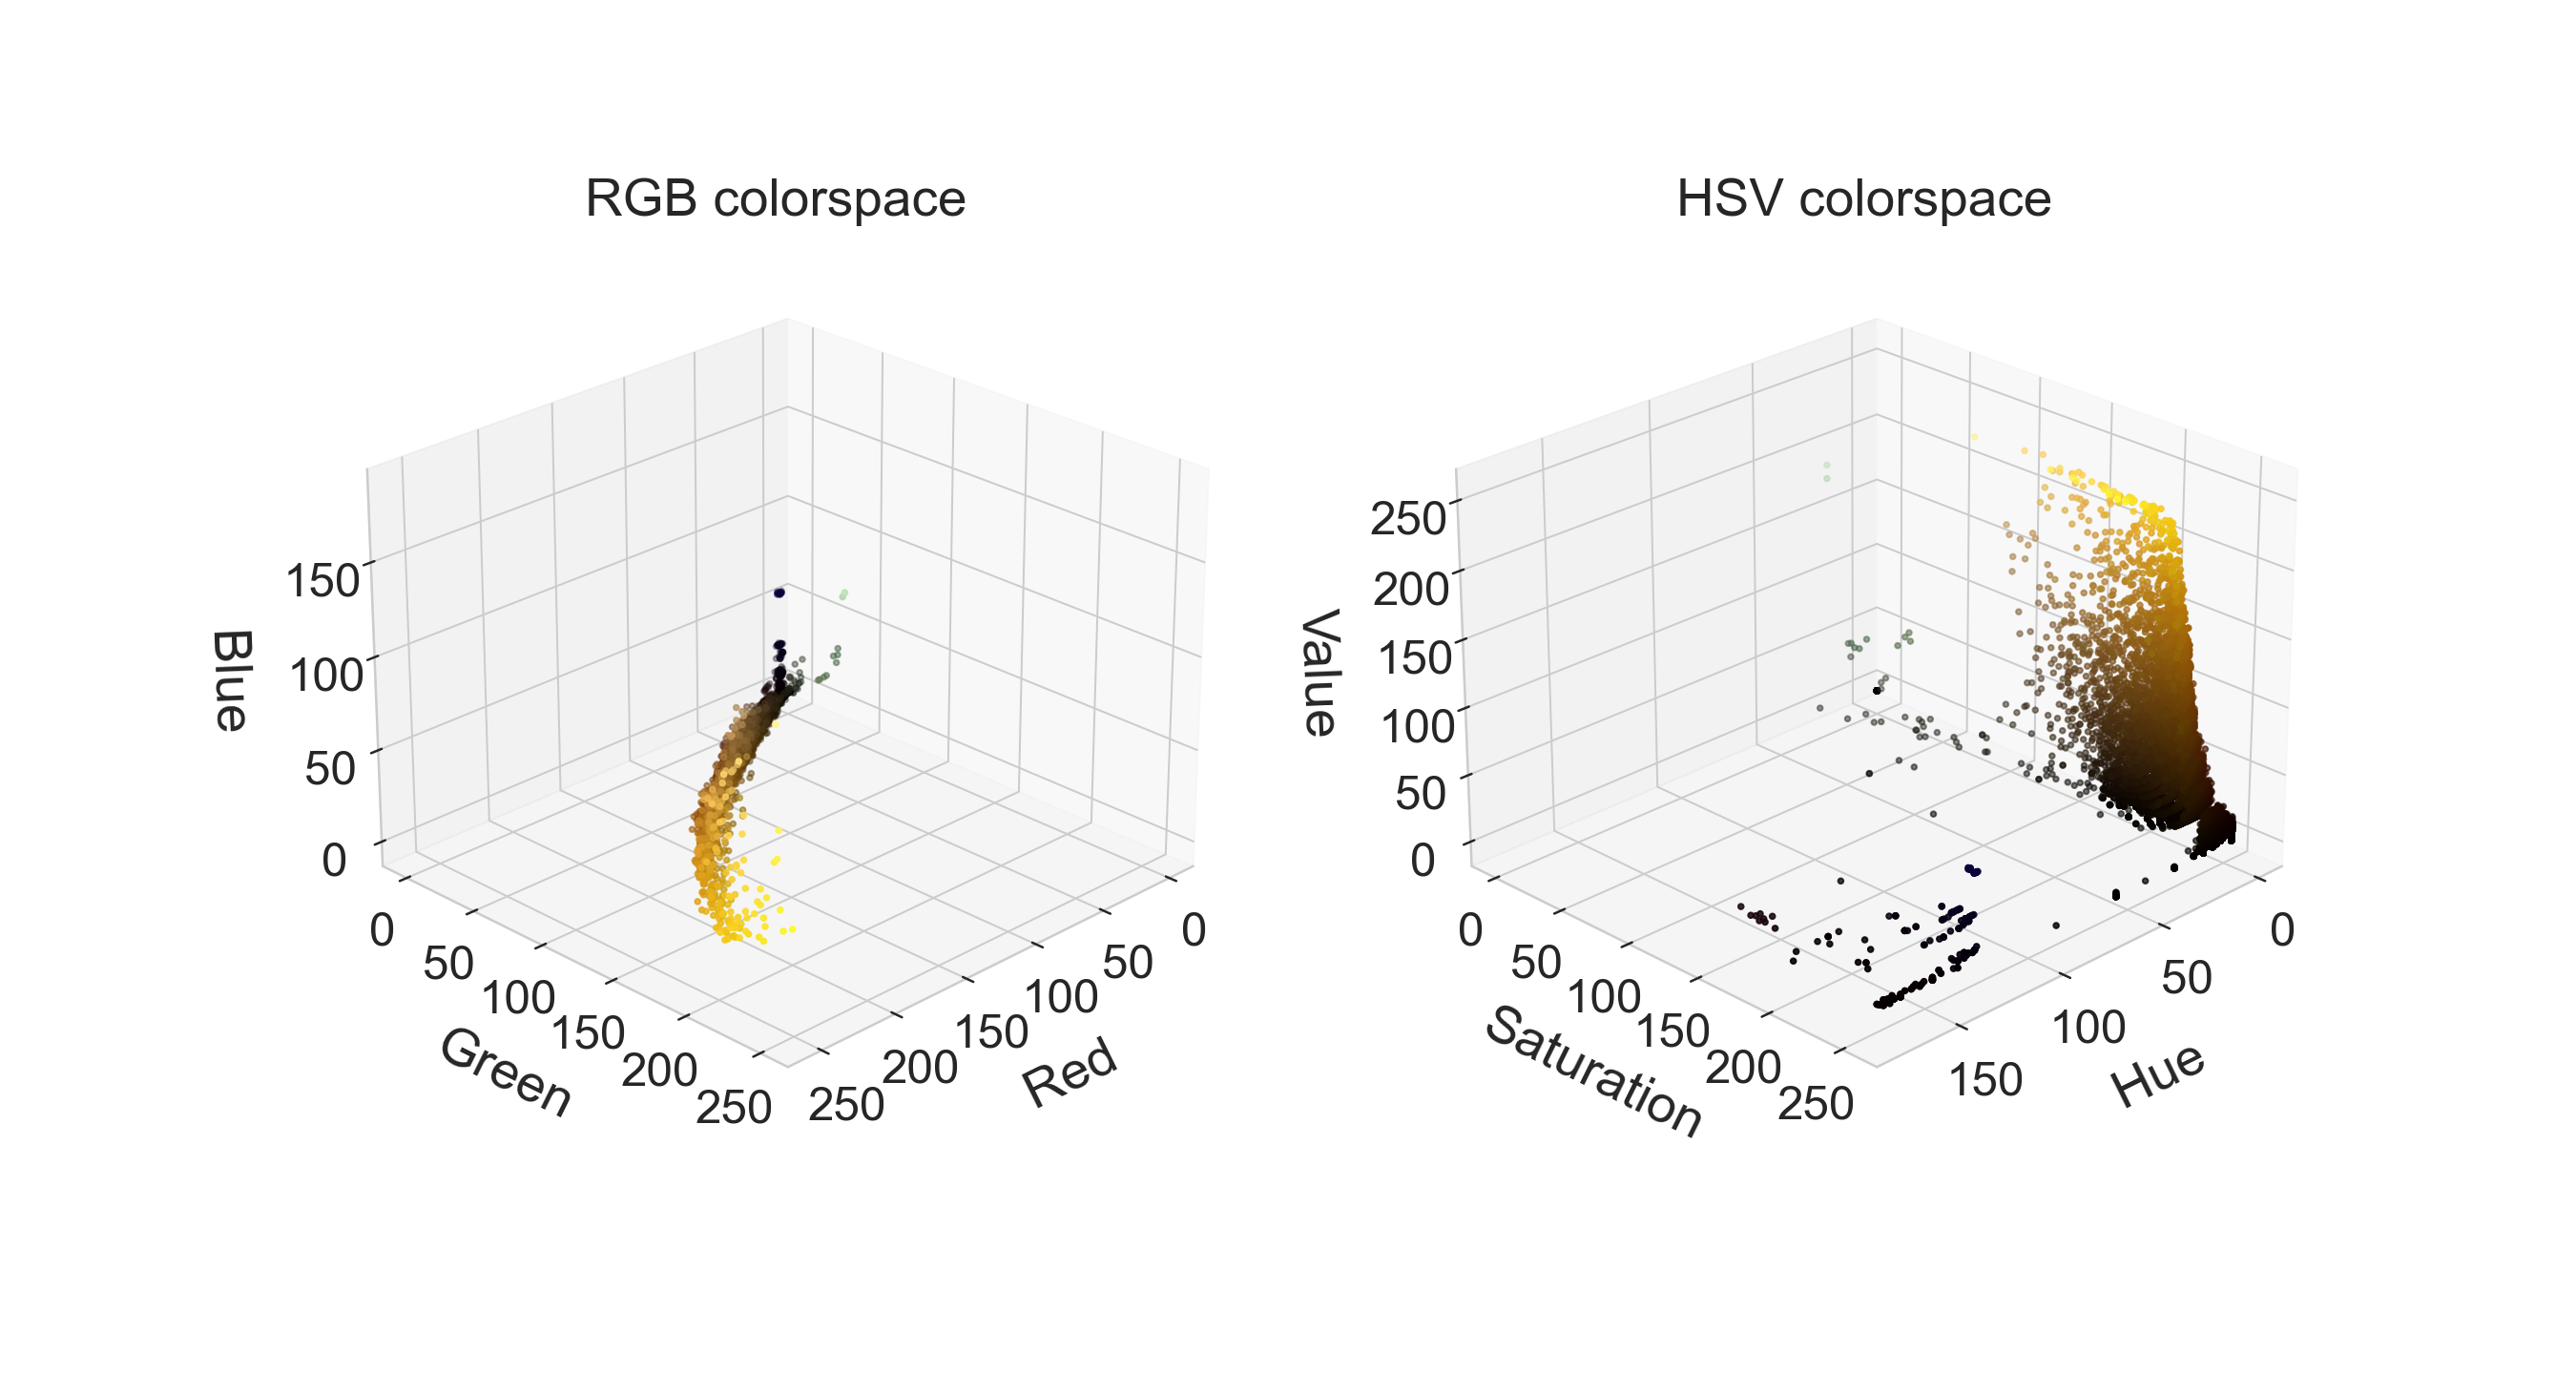
\includegraphics[width=1.1\textwidth]{figures/120_dataset/colorspace_Mar23bS1C2R3_VLPAGl_200x_y.png}
    
%     \centering
%     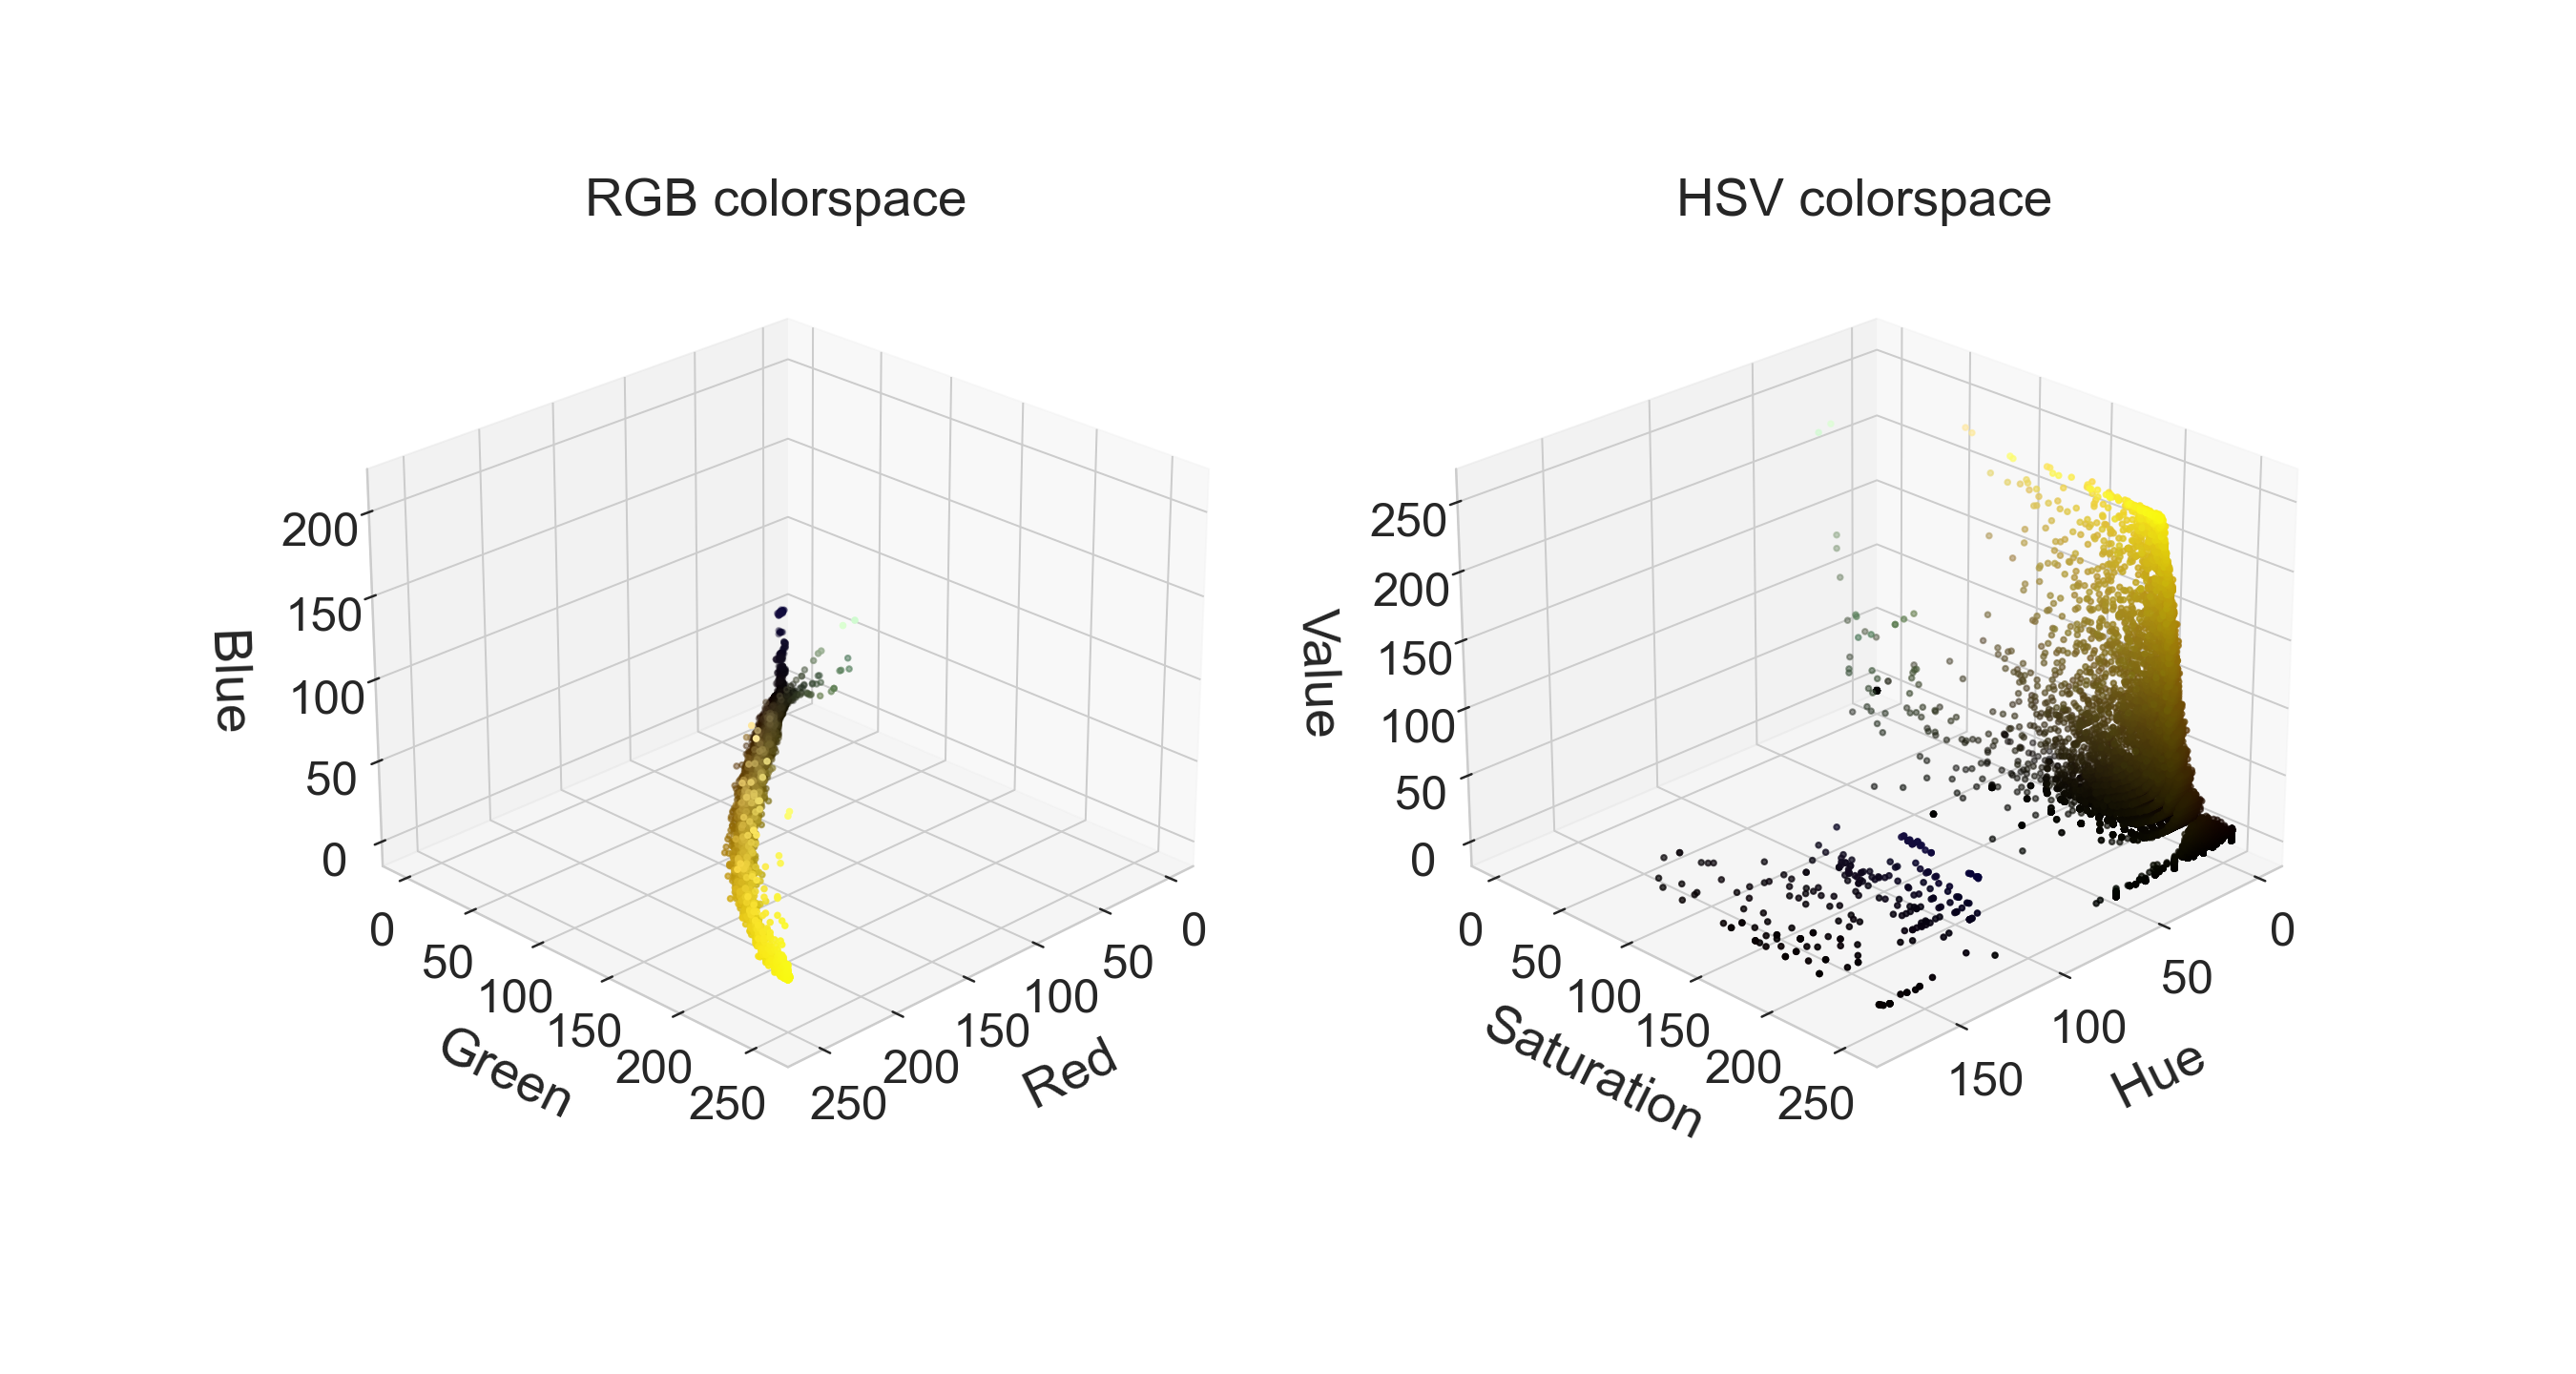
\includegraphics[width=1.1\textwidth]{figures/120_dataset/colorspace_Mar26bS2C1R2_DMl_200x_y.png}
%     \caption{Colorspace representation. The same image is represented as RGB (left) and HSV (right). Pixels are treated as 3D points with coordinates given by their encoding in the corresponding colorspace}
%     \label{fig:dataset:colorspace}
% \end{figure}
% \savegeometry{origigeom}
% \clearpage
% \newgeometry{lmargin=0.5cm}
\begin{figure}

    \centering
    Mar19bS1C4R3\_LHl\_200x\_y.png
    % \vspace{-3cm}
    \makebox[\textwidth][c]{\subfloat[RGB]{
    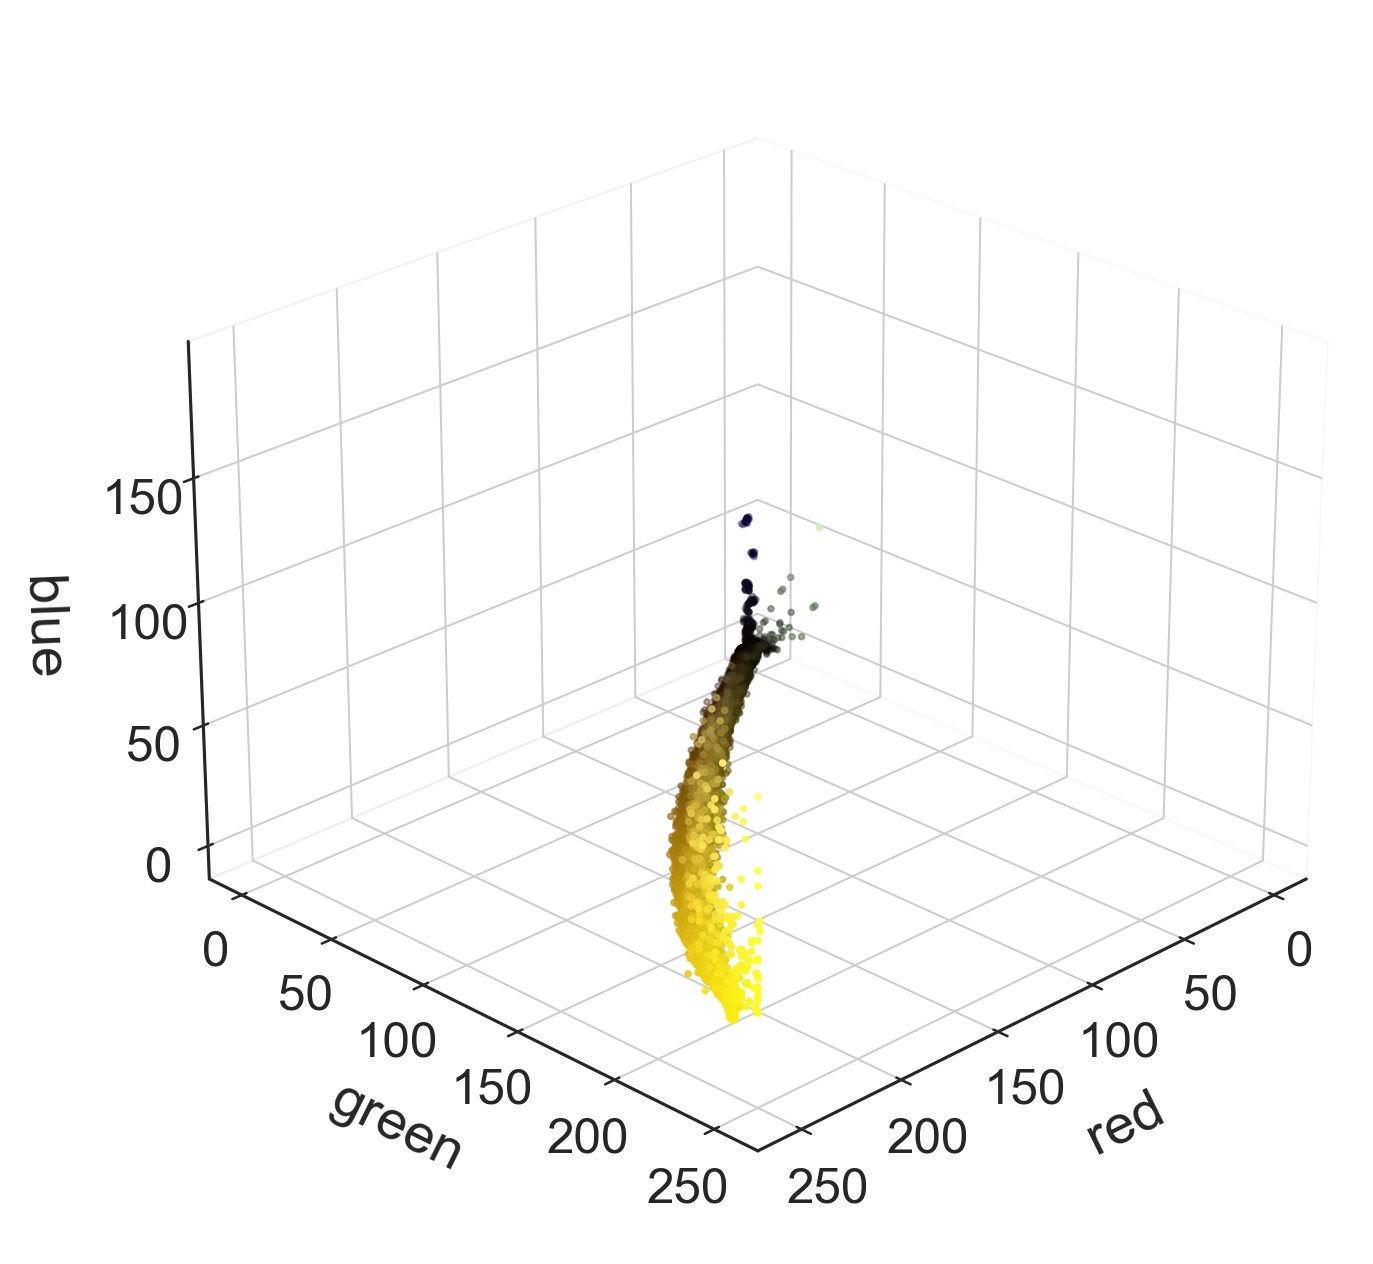
\includegraphics[width=0.55\textwidth]{figures/120_dataset/RGB_Mar19bS1C4R3_LHl_200x_y.png}\label{fig:dataset:colorspace:rgb1}
    }
    \subfloat[HSV]{
    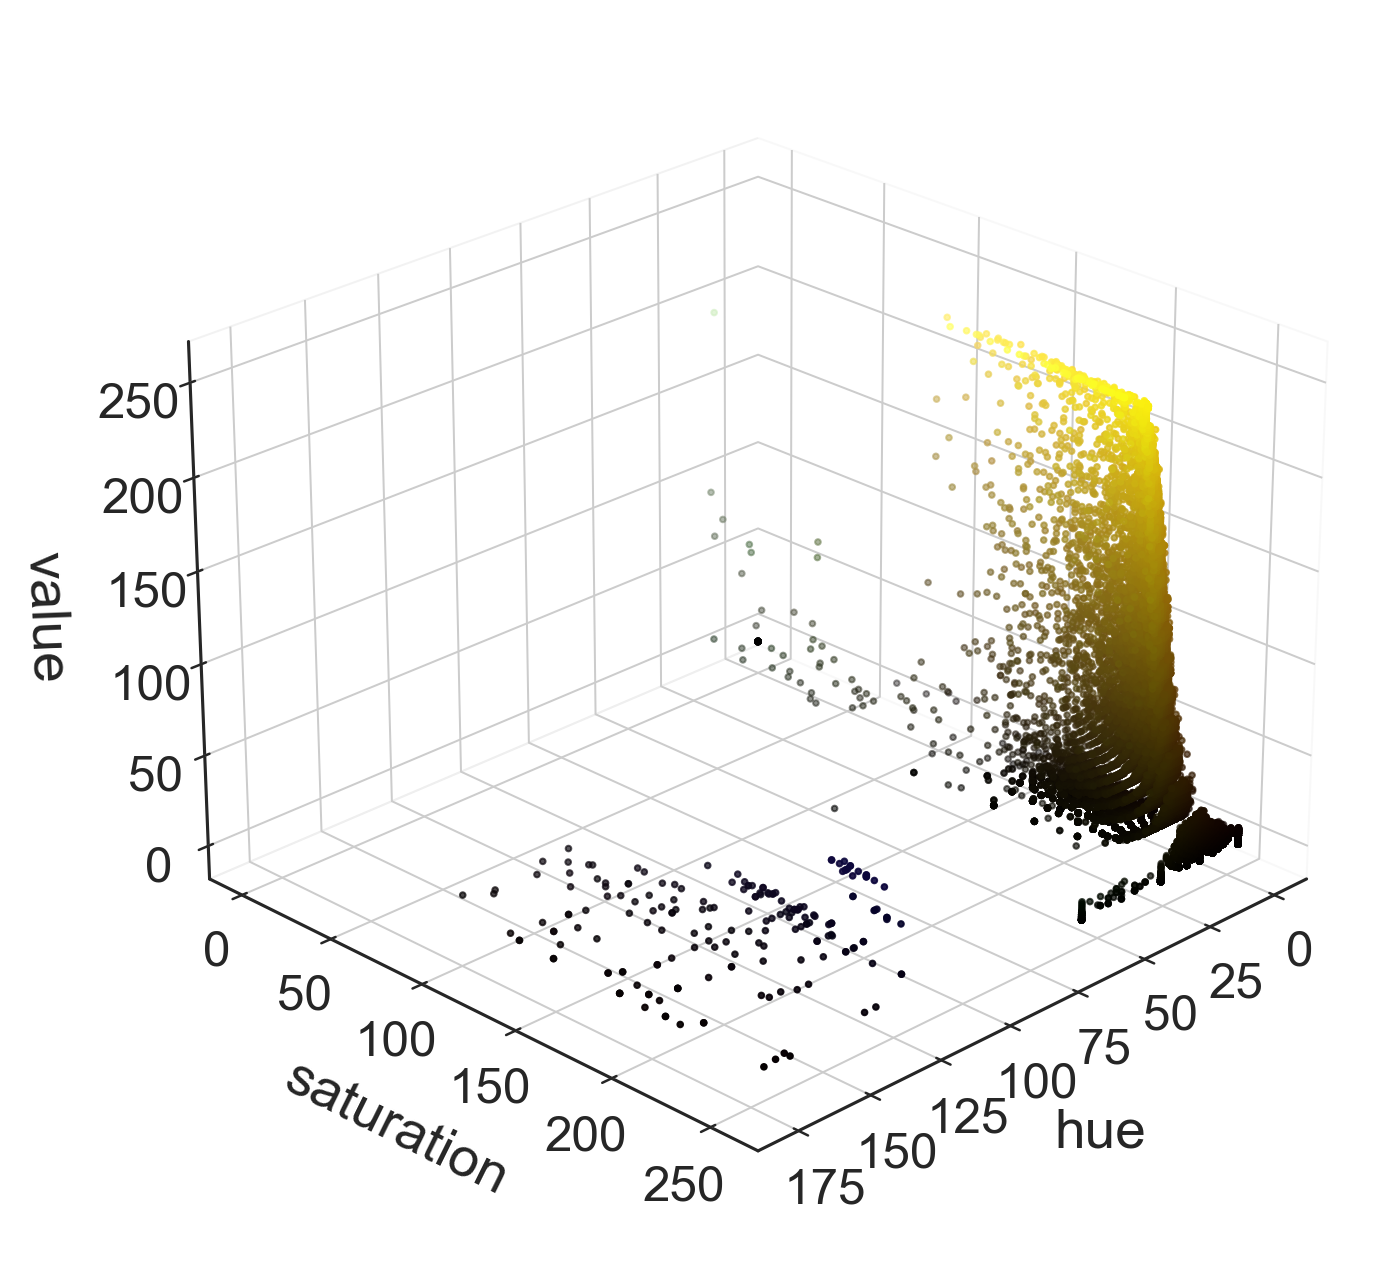
\includegraphics[width=0.55\textwidth]{figures/120_dataset/HSV_Mar19bS1C4R3_LHl_200x_y.png}\label{fig:dataset:colorspace:hsv1}
    }}
    
    \centering
    \vspace{1.5cm}
    Mar21bS1C1R3\_VLPAGl\_200x\_y.png   \makebox[\textwidth][c]{ \subfloat[RGB]{
    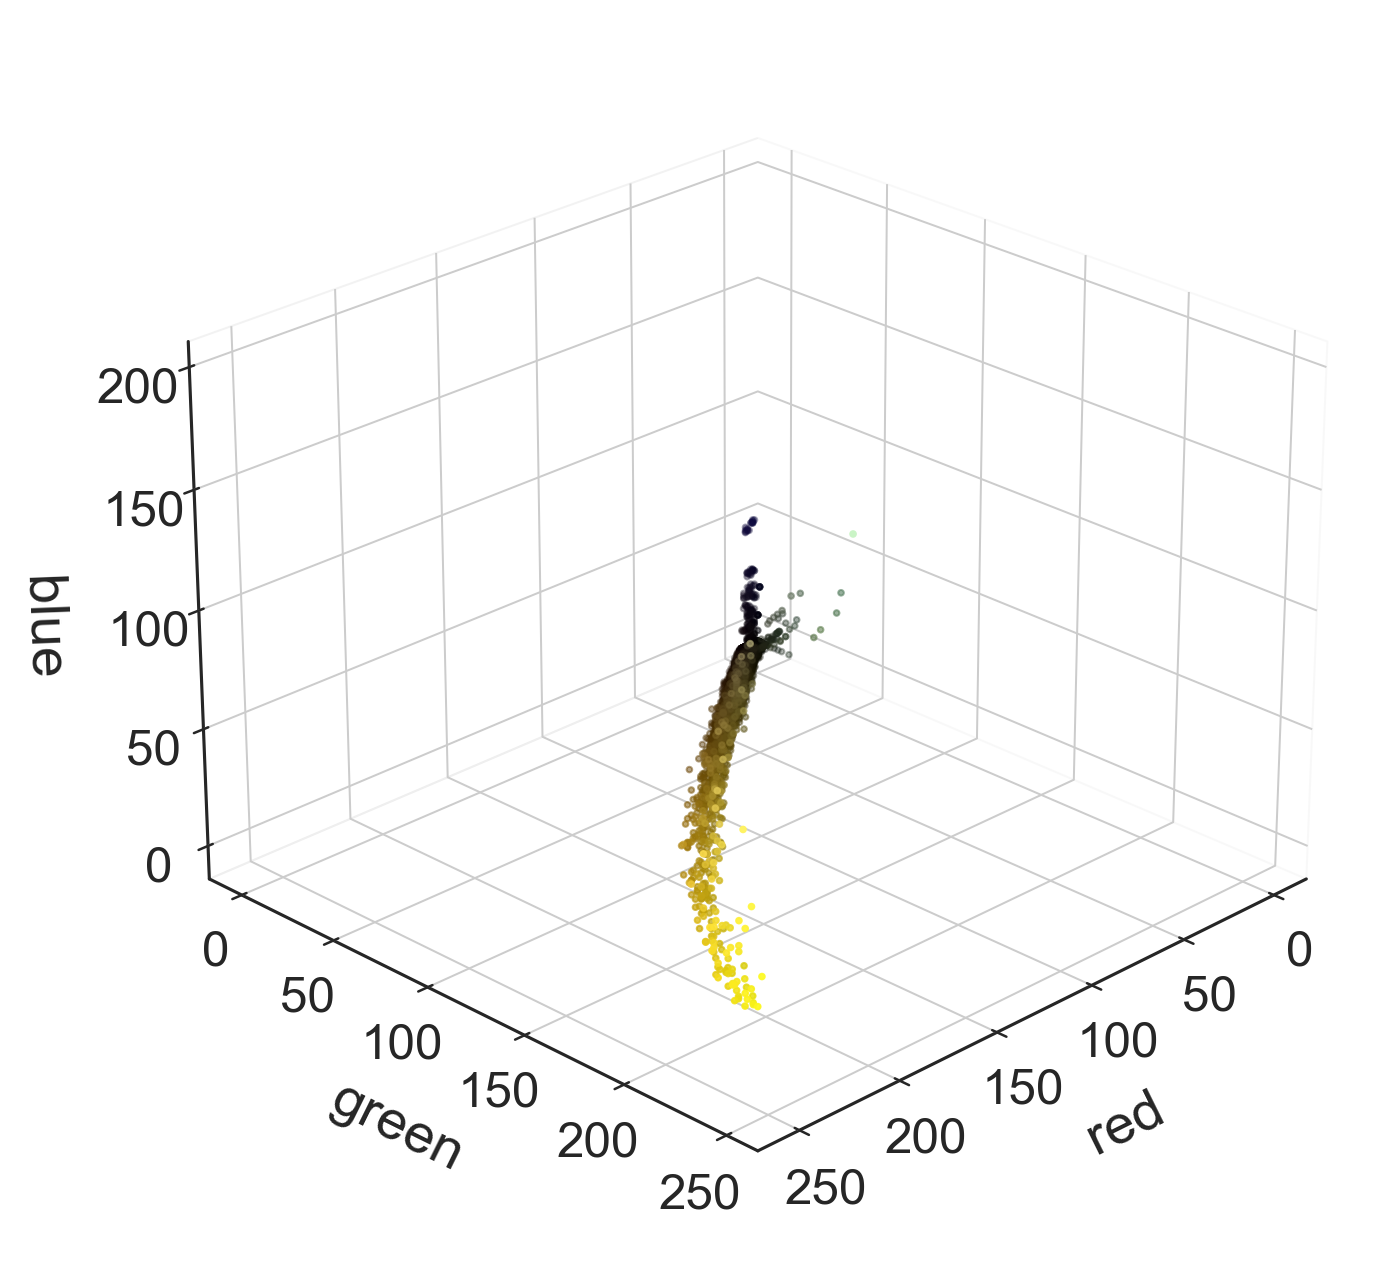
\includegraphics[width=0.55\textwidth]{figures/120_dataset/RGB_Mar21bS1C1R3_VLPAGl_200x_y.png}\label{fig:dataset:colorspace:rgb2}
    }
    \subfloat[HSV]{
    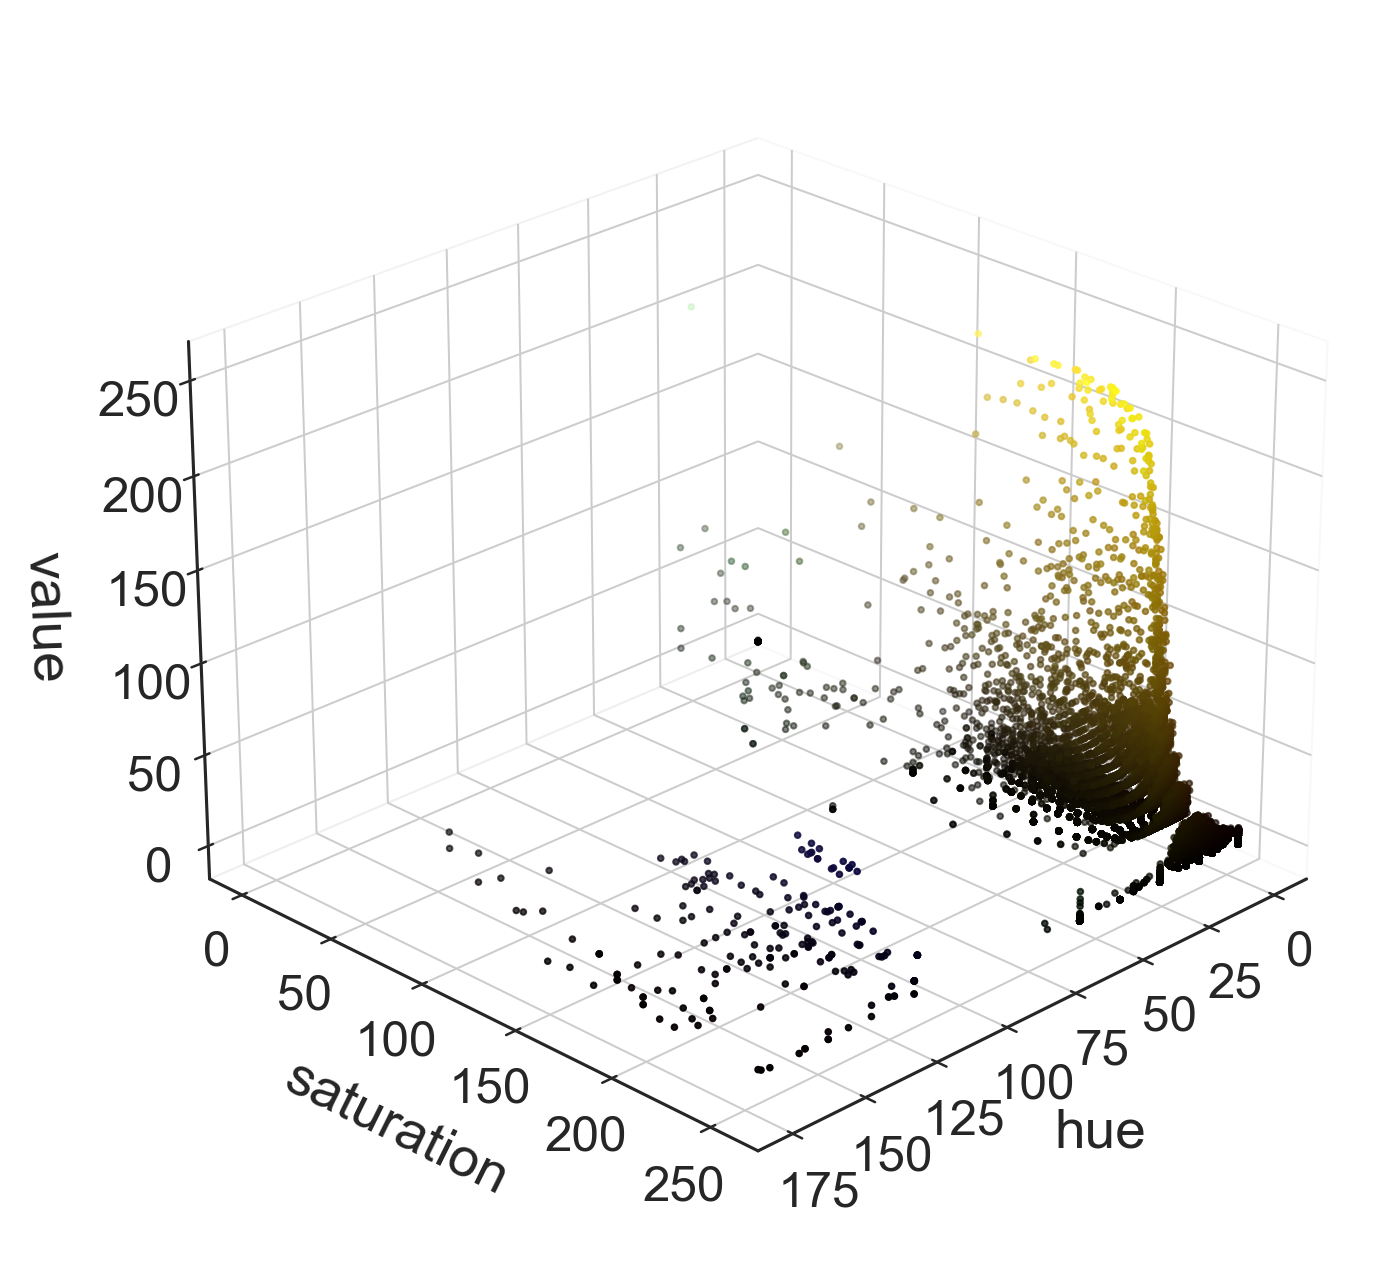
\includegraphics[width=0.55\textwidth]{figures/120_dataset/HSV_Mar21bS1C1R3_VLPAGl_200x_y.png}\label{fig:dataset:colorspace:hsv2}
    }}
    \caption{\textbf{Colorspace.} Two images represented as 3D points according to their RGB (left) and HSV (right) encodings. 
    Each point is colored as the corresponding pixel in the original image
    % The point color is the same as the pixel's color in the original image.
    }
    \label{fig:dataset:colorspace}
\end{figure}

% \clearpage
% \restoregeometry

\subsection{Class imbalance}
\label{sec:class_imbalance}
% \begin{figure}
%     \centering
%     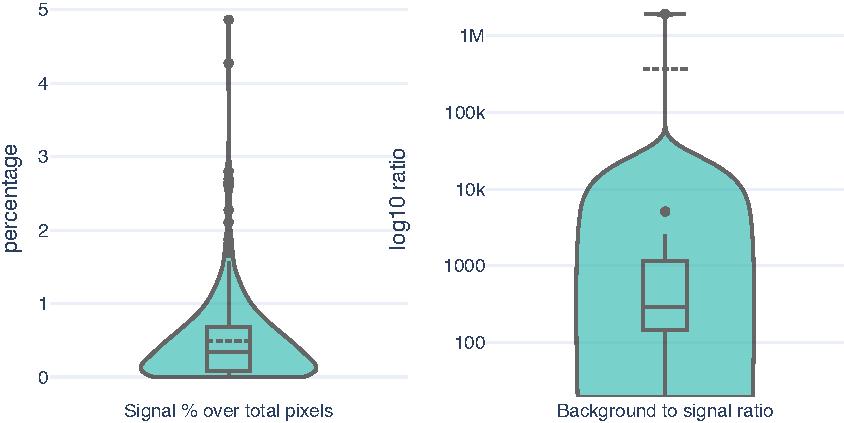
\includegraphics[width=\textwidth]{figures/120_dataset/features/class_imbalance.pdf}
%     \caption{\textbf{Class imbalance.} Violin plot and boxplot of signal percentage (left) and background to signal ration (right).}
%     \label{fig:dataset:class_imbalance}
% \end{figure}
\begin{figure}
    \centering
    \subfloat[Signal \% over total pixels]{
    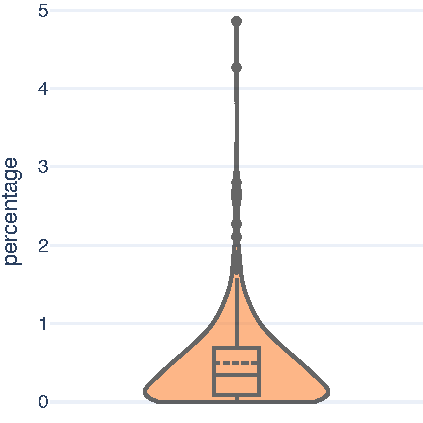
\includegraphics[width=0.5\textwidth]{figures/120_dataset/features/class_imbalance_percentage.pdf}\label{fig:dataset:class_imbalance:percentage}
    }
    \subfloat[Background to signal ratio]{
    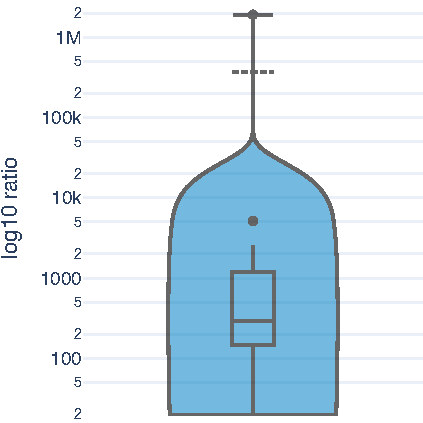
\includegraphics[width=0.5\textwidth]{figures/120_dataset/features/class_imbalance_ratio.pdf}\label{fig:dataset:class_imbalance:ratio}
    }
    \caption{\textbf{Class imbalance.} Violin plot and boxplot of signal percentage (left) and background to signal ration (right).}
    \label{fig:dataset:class_imbalance}
\end{figure}

Inspecting ground-truth masks at pixel level reveals important characteristics that affect the training process. 
By looking at the cardinality of pixels belonging to the background and the signal it is possible to notice how the two classes are extremely unbalanced (see \textit{signal (\%)}, and \textit{signal ratio} columns in \cref{tab:data_features} for a numeric summary).
\Cref{fig:dataset:class_imbalance:percentage} shows a violin plot of the percentage of signal pixel over the total image pixels across the 283 pictures.
The distribution is deeply skewed towards 0, with a median of 0.34\% and a 90\emph{-th} percentile of 1.07\%. 
Hence, almost 90\% of the images contain less than 1\% of pixels belonging to the signal%
% , causing an extreme unbalance between signal and background classes
.
Even more significantly, the right tail does not exceed 5\% of signal coverage, with a maximum of 4.86\%.

\Cref{fig:dataset:class_imbalance:ratio} illustrates the same concept but focuses on the relative proportion of background to signal. 
The distribution is left-skewed, with a lower half concentrated in the range (19, 291), i.e. background pixels are roughly from 20 to 300 times the signal pixels in 50\% of the images.
Remarkably, the disproportion grows even faster in the right tail, where the ratio explodes up to over 1000. 
Finally, notice that the bulk of outliers accumulates in the higher end of the domain. 
This is caused by the contribution of empty masks that cover more than 10\% of the total images.

These considerations expose the need for dedicated training strategies to face this strong class imbalance and correctly learn to classify image pixels.

\subsection{Objects features}
% \begin{figure}
%     \centering
%     \subfloat[Area]{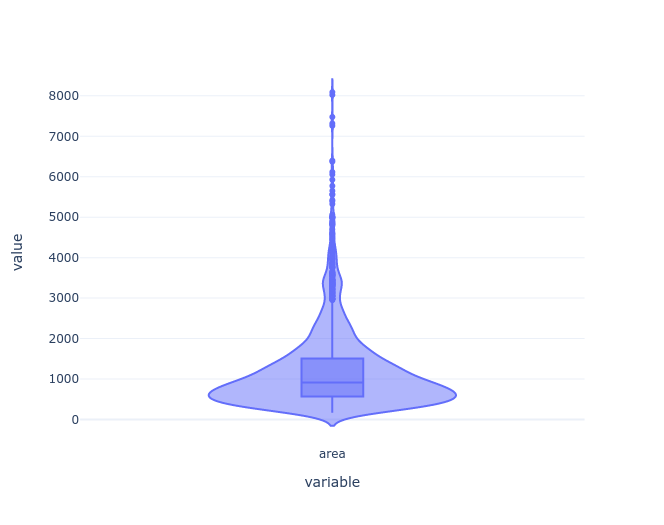
\includegraphics[width=0.5\textwidth]{figures/120_dataset/geometric_features area.png}
%     \label{fig:dataset:geom:area}
%     }
%     \subfloat[Feret diameter]{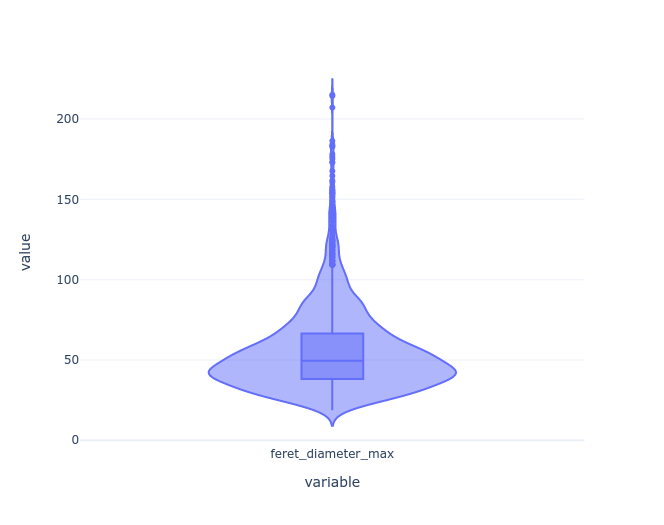
\includegraphics[width=0.5\textwidth]{figures/120_dataset/geometric_features feret.png}
%     \label{fig:dataset:geom:feret}
%     }
%     \caption{\textbf{Geometrical features.} Distributions of the area (left) and maximum Feret diameter (right) across all annotated cells.}
%     \label{fig:dataset:geom}
% \end{figure}
\begin{figure}
    \centering
    \subfloat[Area]{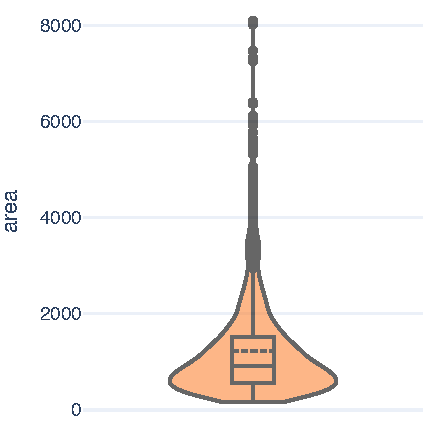
\includegraphics[width=0.5\textwidth]{figures/120_dataset/features/area.pdf}
    \label{fig:dataset:geom:area}
    }
    \subfloat[Feret diameter]{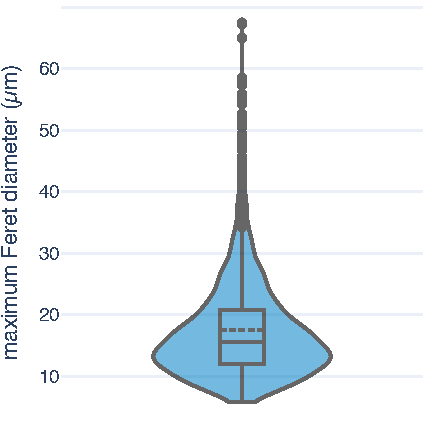
\includegraphics[width=0.5\textwidth]{figures/120_dataset/features/feret_diameter.pdf}\label{fig:dataset:geom:feret}
    }
    \caption{\textbf{Geometrical features.} Distributions of the area (left) and maximum Feret diameter (right) across all annotated cells.}
    \label{fig:dataset:geom}
\end{figure}
After the initial exploration of the data characteristics at the pixel level, additional investigations can be devoted to discovering meaningful insights about images' macroscopic content.
The Fluorescent Neuronal Cells pictures present a rich collection of 2137 neuronal cell instances of various shapes and sizes (see \textit{area}, and \textit{Feret diameter} columns in \cref{tab:data_features} for a numeric summary) that are unevenly distributed across the images.

\Cref{fig:dataset:geom} shows the distributions of the most interesting geometrical features of the annotated objects.
Regarding the area distribution (\cref{fig:dataset:geom:area}), the bulk of the distribution presents cells with a surface within 358 and 1504 pixels.
\Cref{fig:dataset:geom:feret} reports the maximum Feret diameter \cite{merkus2009particle} instead. This measure is computed as the longest distance (in pixels) between points of a convex cell countour\footnote{obtained using skimage package version `0.18.1'}.
The distribution extends from a minimum of 18 to a maximum of 215 pixels, with the central 50\% concentrated in the range [38, 66].
In both cases, the distribution is left-skewed, with a slight prevalence of values lower than the median.
In fact, 90\% of objects are small and medium cells with prevalently regular circular shapes, having an area within [162, 2409] pixels and a Feret diameter between 18 and 88.
The remaining 10\% of the distribution stretches up to a maximum of 8092 and 215, respectively.
This effect is due to the contribution of more oversized or prolonged objects that cause a long, heavy tail.

Finally, \ref{fig:dataset:counts_distrib} illustrates the distribution of the number of cells across the dataset (see \textit{\# cells} columns in \cref{tab:data_features} for a numeric summary).
In this case, the distribution presents multiple modes that can be summed up by the five major peaks, namely 6, 35, 38, 53 and 68
(\cref{fig:dataset:counts_hist}).
The empty spaces are a consequence of the fact that not all of the possible values were actually observed in the data.
Interestingly, a lower peak is observed at 0 because of the 56 images where no cells were annotated.

By looking at the estimated density in the violin plot (\cref{fig:dataset:counts_violin}), it appears that the distribution can be interpreted as a mixture of two components.
%In particular, one can distinguish two peaks by looking at the estimated density in \cref{fig:dataset:counts_violin}.
The first is centered around 6 and is made of the images with lower counts, i.e. the ones depicting brain areas where the fluorophore did not yield abundant emissions.
The second, instead, is a combination of the four higher peaks that represent active brain areas.
% \begin{figure}
%     \centering
%     \subfloat[Histogram]{
%     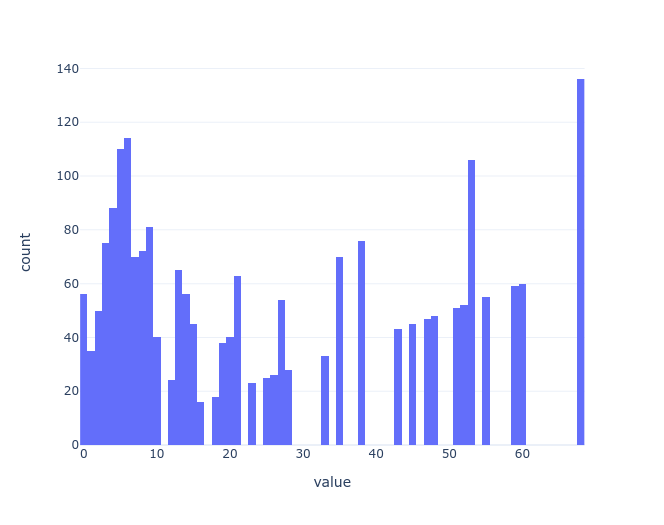
\includegraphics[width=0.5\textwidth]{figures/120_dataset/counts_histogram.png}
%     \label{fig:dataset:counts_hist}
%     }
%     \subfloat[Violin plot]{
%     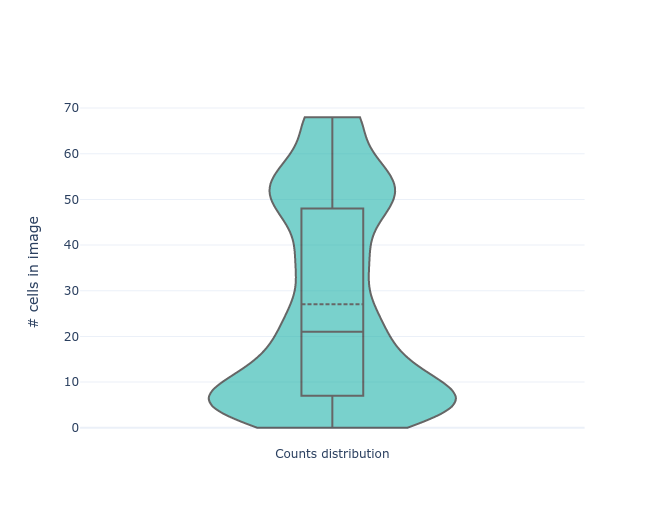
\includegraphics[width=0.5\textwidth]{figures/120_dataset/counts_violin.png}
%     \label{fig:dataset:counts_violin}
%     }
%     \caption{\textbf{Counts distribution.} Distributions of the number of annotated cells across all images in the dataset.}
%     \label{fig:dataset:counts_distrib}
% \end{figure}


\begin{figure}
    \centering
    \subfloat[Histogram]{
    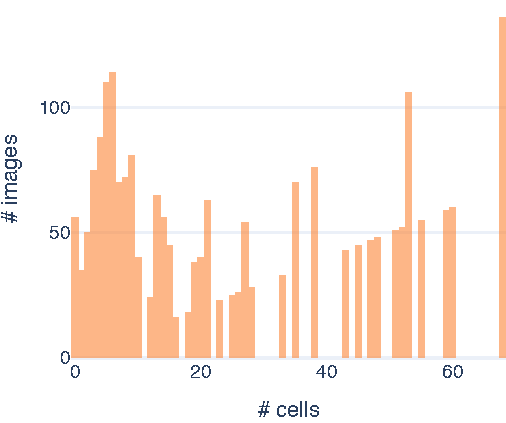
\includegraphics[width=0.6\textwidth]{figures/120_dataset/features/count_histogram.pdf}
    \label{fig:dataset:counts_hist}
    }
    \subfloat[Violin plot]{
    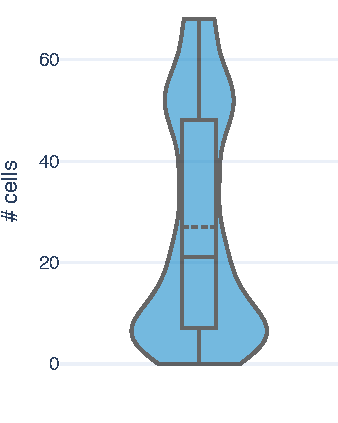
\includegraphics[width=0.4\textwidth]{figures/120_dataset/features/count_violin.pdf}
    \label{fig:dataset:counts_violin}
    }
    \caption{\textbf{Counts distribution.} Distributions of the number of annotated cells across all images in the dataset.}
    \label{fig:dataset:counts_distrib}
\end{figure}

\section{Ground-truth labels}
Under a supervised learning framework, the training phase leverages ground-truth labels acting as examples of desired outputs that the model should learn to reproduce. 
In the case of image segmentation, such targets are in the form of binary images (\textit{masks}) where the objects to segment and the background are represented by white and black pixels, respectively (Fig. \ref{fig:dataset}, right).

Obtaining target masks usually requires a great effort in terms of time and human resources, so an initial automatic procedure was exploited to speed up the labeling process. 
In particular, starting from a large subset composed by 252 pictures, gaussian blurring was first applied to mitigate small-frequency noise. 
Then, the resulting images were subjected to a thresholding operation.
% using a cutoff selected base on the pixel intensity histogram shape. 
For this step, the image histogram of the pixel intensity was considered, and a cutoff equal to the 97\emph{-th} percentile of the intensity distribution was adopted for binarization. 
The goal was to obtain a loose selection of good candidates to be labeled as neuronal cells. 
After that, acknowledged operators reviewed the results to discard the false positives introduced with the previous procedure, taking care of excluding irrelevant artifacts and misleading biological structures.
The remaining 31 images were segmented manually by domain experts. Significant pictures with peculiar traits -- such as artifacts, filaments and crowded objects -- were included in the latter set to have highly reliable masks for the most challenging examples\footnote{check the \emph{README} file in \citeA{clissa2021fluocells} for a detailed list of manually segmented images}. 
% (see $link_to_github$ for more details).

% \lc{A summary of the distributions of counts and objects features is presented in Table \ref{tab:dataset_summary}}.
% % ...possibly add geometrical information of cell objects, average/median/max/min counts per image, ... others(?)
% \begin{table}[b]
% \begin{center}
% \begin{tabular}{cccccc}
% \hline
% area    & minor axis & major axis & equivalent diameter & maximum feret diameter & mean diameter \\
% \hline
% 1206.43 & 29.39 & 50.43 & 36.50 & 55.34 & 47.42\\
% \hline
% \end{tabular}
% \caption{Summary statistics of cells morphological features (measured in pixels)}
% \label{tab:dataset_summary}
% \end{center}
% \end{table}


Despite the huge popularity Deep Learning has gained in computer vision in the last decade, the lack of annotated data is a common curse when dealing with applications involving non-standard pictures and/or tasks \cite{curse_dataset_annotation}. 
Since ground-truth labels are expensive to acquire in terms of time and costs \cite{vija2009annotationcost, mullen2019comparing}, a common approach is to fine-tune models pre-trained on giants datasets of natural images like ImageNet \cite{ImageNet} or COCO \cite{COCO}, possibly using as few new labels as possible for the task of interest. 
However, this strategy often does not apply to use cases where the pictures under analysis belong to extraneous domains with respect to the ones used for pre-training \cite{TL_medical_imaging}.
For this reason, by releasing the annotated dataset\footnote{\dataset} and the pre-trained model\footnote{\linkmodel} we hope to \textit{i)} foster advances in fields like biomedical imaging through the speed up guaranteed by the automation of manual operations, and \textit{ii)} promote methodological research on new techniques of data analysis for microscopic fluorescence and similar domains.


\section{Challenges}

% Although many efforts were made to stabilize the acquisition procedure, the images present several relevant challenges for the detection task. 
% For example, the variability in brightness and contrast causes some fickleness in the pictures overall appearance (cfr. \cref{fig:dataset:dark,fig:dataset:bright}).  
% Also, the cells themselves exhibit varying saturation levels due to the natural fluctuation of the fluorescent emission properties (cfr. \cref{fig:dataset:dark,fig:artifacts:clumping}).
% Moreover, the substructures of interest have a fluid nature. This implies that the size and shape of the stained cells may change significantly (see \cref{fig:artifacts:clumping}, right), making it even harder to discriminate between them and the background. 
% Combined to that, artifacts (\cref{fig:artifacts:stripe,fig:artifacts:macaroon}), bright biological structures -- like neurons' filaments -- (\cref{fig:artifacts:stripe}) and non-marked cells similar to the stained ones handicap the recognition task. 
% Last but not least, another source of complexity is the broad shift in the number of target cells from image to image.
% Indeed, the total counts range from no stained cells (\cref{fig:dataset:empty}) to several dozens clumping together (\cref{fig:artifacts:clumping}). 
% As a consequence, this requires a model with both high precision -- to prevent false positives in the former case -- and high recall -- since considering two or more touching neurons only once produces false negatives.
% % In the former case, the model needs high precision in order to prevent false positives. The latter, instead,
% % requires high recall since considering two or more touching neurons only once produces false negatives. 

% \note[Luca][notesyellow]{Aggiungere unbalanced dataset}

Although many efforts were made to stabilize the acquisition procedure, the images present several relevant challenges for the detection task. 

Graphical properties of the pictures are undoubtedly valuable information for the classification of the pixels. However, that alone is not enough.
Indeed, an elementary approach would be to apply selection cuts over these features to separate cell pixels from the background.
Nonetheless, the characterization of cells in terms of color, saturation and contrast varies from image to image, making it difficult to generalize hard-coded thresholds.
For example, the tissues can sometimes soak in some of the marker, causing irrelevant compounds to emit light which is then captured by the microscope. 
When that is the case, the background assumes a similar hue to the neuronal cells (cfr. \cref{fig:dataset:dark,fig:dataset:bright}), and the identification falls back to other characteristics such as saturation and contrast.
In addition to that, fluorescent emissions are naturally unstable, thus generating fluctuations of the saturation levels exhibited by pixels belonging to cells (cfr. \cref{fig:dataset:dark,fig:artifacts:clumping}).

Moreover, the substructures of interest have a fluid nature. This implies that the size and shape of the stained cells may change significantly (see \cref{fig:artifacts:clumping}, right and \cref{fig:dataset:geom_area}), making it even harder to discriminate between them and the background.

Another challenge is represented by artifacts, i.e. fictitious objects accidentally present in pictures which resemble neuronal cells in terms of shape, size or color.
One example is when the marker forms accumulations of fluorophore in narrow areas that generate emissions very similar to the ones of the cells. In such cases, thresholding becomes ineffective and one has to resort to physiological characteristics as cells' shape and size in order to distinguish them from such artifacts.
Nevertheless, the distinction is not always unambiguous and this poses an issue of intrinsic subjectivity in the annotation process, which is then reflected on model performance.

A further source of complexity is represented by the broad shift in the number of target cells from image to image.
Indeed, the total counts range from no stained cells (\cref{fig:dataset:empty}) to \sidenote[Luca][notesyellow]{approfondire meglio per giustificare ablations study...magari inserendo più immagini come esempi di overcrowding}several dozens clumping together (\cref{fig:artifacts:clumping}). 
As a consequence, this requires a model with both high precision -- to prevent false positives in the former case -- and high recall -- since considering two or more touching neurons only once produces false negatives.

Last but not least, the objects are typically small and cover only marginal portions of the images. This generates an extreme imbalance between signal and background, which is even worsened by the high resolution of the pictures.
Hence, dedicated learning strategies are demanded to mitigate this issue during the training phase.

By and large, all of these factors make the recognition and counting tasks more problematic and complicate the learning process.
Likewise, borderline annotations hinder model evaluation as their subjectivity deprives the model of a reliable and indisputable testbed.